%% ****** Start of file aiptemplate.tex ****** %
%%
%%   This file is part of the files in the distribution of AIP substyles for REVTeX4.
%%   Version 4.1 of 9 October 2009.
%%
%
% This is a template for producing documents for use with 
% the REVTEX 4.1 document class and the AIP substyles.
% 
% Copy this file to another name and then work on that file.
% That way, you always have this original template file to use.

%\documentclass[aip,graphicx]{revtex4-1}
%\documentclass[aip,reprint]{revtex4-1}

%\usepackage{graphicx}

%\draft % marks overfull lines with a black rule on the right
%\documentclass[pre,aps,floatfix,authordate1-4,twocolumn]{revtex4-1}
%\documentclass[pre,aps,floatfix,authordate1-4]{revtex4-1}

\documentclass[aps,prl,superscriptaddress,twocolumn]{revtex4}



%\documentclass[aps,prl,preprint,groupedaddress]{revtex4}

\usepackage{rotating} 
\usepackage{times}
\usepackage{graphicx}
\usepackage{setspace}
\usepackage{amsmath}
\usepackage{epstopdf}
\usepackage[obeyFinal]{easy-todo}
\usepackage{csquotes}
\usepackage{xr}
\externaldocument{manuscriptPSsuppl}

\begin{document}

% Use the \preprint command to place your local institutional report number 
% on the title page in preprint mode.
% Multiple \preprint commands are allowed.
%\preprint{}

\title{NMRlipids IV: Headgroup \& glycerol backbone structures, and cation binding in bilayers with PS lipids} %Title of paper

% repeat the \author .. \affiliation  etc. as needed
% \email, \thanks, \homepage, \altaffiliation all apply to the current author.
% Explanatory text should go in the []'s, 
% actual e-mail address or url should go in the {}'s for \email and \homepage.
% Please use the appropriate macro for the type of information

% \affiliation command applies to all authors since the last \affiliation command. 
% The \affiliation command should follow the other information.

\author{Pavel Buslaev}
\affiliation{Moscow Institute of Physics and Technology}
\author{Tiago M. Ferreira}
\affiliation{Halle, Germany}
\author{Ivan Gushchin}
\affiliation{Moscow Institute of Physics and Technology}
\author{Matti Javanainen}
\affiliation{Institute of Organic Chemistry and Biochemistry,
Academy of Sciences of the Czech Republic, 
Prague 6, Czech Republic}
\author{Batuhan Kav}
\affiliation{Potsdam, Germany}
\author{Jesper J. Madsen}
\affiliation{Department of Chemistry, The University of Chicago, Chicago, Illinois 60637, United States of America}
\author{Markus Miettinen}
\affiliation{Potsdam, Germany}
\author{Josef Melcr}
\affiliation{Institute of Organic Chemistry and Biochemistry,
Academy of Sciences of the Czech Republic, 
Prague 6, Czech Republic}
\author{Ricky Nencini}
\affiliation{Institute of Organic Chemistry and Biochemistry,
Academy of Sciences of the Czech Republic, 
Prague 6, Czech Republic}
\author{O. H. Samuli Ollila}
\email[]{samuli.ollila@helsinki.fi}
%\homepage[]{Your web page}
\affiliation{Institute of Organic Chemistry and Biochemistry,
Academy of Sciences of the Czech Republic, 
Prague 6, Czech Republic}
\affiliation{Institute of Biotechnology, University of Helsinki}
\author{Thomas Piggot   \todo{Authorlist is not yet complete}}
\affiliation{Southampton, United Kingdom}
%\author{NMRlipids collaboration}
%\affiliation{nmrlipids.blogspot.fi} 


% Collaboration name, if desired (requires use of superscriptaddress option in \documentclass). 
% \noaffiliation is required (may also be used with the \author command).
%\collaboration{}
%\noaffiliation

\date{\today}

\begin{abstract}
  % insert abstract here
Phosphatidylserine (PS) is the most common negatively
charged lipid in eykaryotic membranes.
PS lipids interact with signaling and other proteins via
electrostatic interactions and direct binding, and induce
membrane fusion and phase separation together with calcium ions.
Molecular details of these phenomena are not well understood
because accurate models to interpret the experimental data has not
been available. Here, we collect a set of experimental NMR data which
can be used together with molecular dynamics (MD) simulations
to interpret the lipid headgroup structures and details of ion binding
in pure PS and mixed PS:PC lipid bilayers. We use the open collaboration
method to collect data from available MD simulation models of PS lipids.
None of the models reproduce the NMR data with experimental accuracy,
but the best models suggest that the carboxyl group in the serine headgroup
does not rotate freely. In line with the previous results for PC lipids,
all the tested force fields overestimate the cation binding affinity to lipid bilayers containing
PS lipids. In contrast to PC lipids, the response of PS headgroups
to the bound ions qualitatively differs from experiments in the tested MD
simulation models. The collected experimental dataset and simulation
results pave the way for improvement of lipid force fields to correctly
describe negatively charged membranes and their interactions with ions.
The work is performed in the NMRlipids open collaboration project (\url{nmrlipids.blogspot.fi}).
\end{abstract}

%\pacs{}% insert suggested PACS numbers in braces on next line

\maketitle %\maketitle must follow title, authors, abstract and \pacs

% Body of paper goes here. Use proper sectioning commands. 
% References should be done using the \cite, \ref, and \label commands


%\label{}
\section{Introduction}
Phosphatidylserine (PS) is the most common negatively
charged lipid in eykaryotic membranes.
PS lipids compose 8.5\% of total lipid weight of erythrocytes,
but the abundance varies between different organelles up to
25-35\% in plasma membrane \cite{lemmon08,leventis10,li14}.
Despite of the relatively low abundance, PS lipids
are important signaling molecules. They interact with
signaling proteins \cite{leventis10}, regulate
surface charge and protein localization \cite{yeung08}, and
induce protein aggregation \cite{zhao04,gorbenko06}.
Some domains spesifically interact PS lipids,
while others are attracted by general electrostatics and the
binding can be regulated by calcium \cite{leventis10}.
Therefore, the structural details
of lipid headgroups and the details of cation binding
are crucial for the PS mediated signaling processes.

Previous experimental studies have concluded that
PS headgroups are more rigid than phophocholines (PC)
due to the hydrogen bonding network or
electrostatic interactions \cite{browning80,buldt81}.
Multivalent cations and Li$^+$ are able to form strong
dehydrated molecular complexes with PS lipids,
while monovalent ions interact more weakly with PS
containing bilayers \cite{hauser77,kurland79,eisenberg79,hauser83,dluhy83,hauser85,feigenson86,mattai89,roux90,roux91,boettcher11}.
The dehydrated complexes of PS headgroup and calcium ions can also lead to the
phase separation \cite{hauser77,kurland79,hauser85,feigenson86,mattai89,roux90,roux91}.
On the other hand, some studies propose that the specific binding
affinity is similar to the negatively charged and zwitterionic lipids and that
the increased cation binding to negatively charged lipid bilayer arise only due
to the increase of local cation concentration in the vicinity of membranes \cite{seelig90,sinn06}.
Dilution of bilayers with PC lipids makes PS headgroups
less rigid and reduces propensity for the formation of
strong complexes with multivalent ions \cite{browning80,buldt81,roux90,roux91}.
The molecular level interpretation of these observations is,
however, not available.

Several classical molecular dynamics (MD) simulation studies are done
to understand PS headgroups, their influence on lipid bilayer properties and
interactions with
ions \cite{cascales96,pandit02,mukhopadhyay04,pedersen06,vernier09,boettcher11,molina12,jurkiewicz12,venable13,pan14,vangaveti14,melcrova16,valentine18}.
However, the headgroup structures and ion binding affinity 
predicted by the MD simulation force fields for bilayers containing PS lipids are not
evaluated against experiments. Recent studies comparing the
C-H bond order parameters between simulations and experiments show that the
structure of PC lipid headgroup and glycerol backbone are not well
captured by most simulation models \cite{botan15} and that the cation binding to PC
lipid bilayers is overestimated \cite{catte16}. Based on this data,
the cation binding affinity to POPC bilayer was then improved by implicitly
including the electronic polarizability using the electronic continuum correction \cite{melcr18}.

\begin{table*}[htb]
%\begin{sidewaystable*}[!p]
\centering
\caption{The list of MD simulations of pure PS bilayers without additional salt.
  Simulation details are given in the supplementary information
    %   The lipid force fields named as in our previous work~\cite{botan15}.
}\label{PSsystems}
%begin{minipage}[t]{\textwidth}
\begin{tabular}{l c r r r r r c c}
  %\hline
  % some footnotes are not visible in typeset-MS (pdf)
 lipid/counter-ions & force field for lipids / ions & \footnote{Number of lipid molecules with largest mole fraction}N$_{\rm l}$   &  \footnote{Number of water molecules}N$_{\rm w}$  & \footnote{Number of additional cations}N$_{\rm c}$  & \footnote{Simulation temperature}T (K)  & \footnote{Total simulation time}t$_{{\rm sim}}$(ns) & \footnote{Time used for analysis}t$_{{\rm anal}}$ (ns) &   \footnote{Reference for simulation files}files\\
  \hline
    DOPS/Na$^+$  & CHARMM36 \cite{venable13}       & 128 & 4480 & 0  & 303  & 500 & 100 & \cite{charmm36DOPS303K} \\
    DOPS/Na$^+$  & CHARMM36ua \cite{??} \todoi{Correct citation for CHARMMua DOPS}   & 128 & 4480 & 0  & 303  & 500 & 100 & \cite{charmm36uaDOPS303K} \\
    DOPS/Na$^+$  & Slipids \cite{jambeck13}        & 128 	& 4480  & 0  & 303  & 500 & 100 & \cite{slipidsDOPS303K} \\
    DOPS/Na$^+$  & Slipids \cite{jambeck13}        & 288 	& 11232 & 0  & 303  & 200 & 100 & \cite{slipidsDOPSfiles} \\
    DOPS/Na$^+$  & Berger \cite{mukhopadhyay04}    & 128  & 4480  & 0  & 303  & 500 & 100 & \cite{bergerDOPS303K} \\
    DOPS/Na$^+$  & GROMOS-CKPM \cite{??} \todoi{Correct citation(s) for CKP.} & 128 & 4480 & 0  & 303  & 500 & 100 & \cite{ckp1DOPS303K} \\
    DOPS/Na$^+$  & GROMOS-CKP  \cite{??} \todoi{Correct citation(s) for CKP.} & 128 & 4480 & 0  & 303  & 500 & 100 & \cite{ckp2DOPS303K} \\
    DOPS/Na$^+$  & lipid17 \cite{gould18} / JC  \cite{joung08}    & 128    & 4480   & 0   & 303  & 600 & 100 & \cite{lipid17DOPSjcions} \\
    DOPS/Na$^+$  & lipid17 \cite{gould18} / ff99 \cite{aqvist90}  & 128    & 4480   & 0   & 303  & 600 & 100 & \cite{lipid17DOPSff99ions} \\
    \hline
    POPS/Na$^+$  & CHARMM36 \cite{venable13} & 128 & 4480 & 0  & 298  & 500 & 100 & \cite{charmm36POPS298K} \\
    POPS/K$^+$   & CHARMM36 \cite{venable13} & 128 & 4480 & 0  & 298  & 500 & 100 & \cite{charmm36POPS298Kpotassium} \\
    POPS/Na$^+$  & CHARMM36ua \cite{??} \todoi{Correct citation for CHARMMua DOPS} & 128 & 4480 & 0  & 298  & 500 & 100 & \cite{charmm36uaPOPS298K} \\
    POPS/Na$^+$  & Slipids \cite{jambeck13}  & 128 & 4480 & 0  & 298  & 500 & 100 & \cite{slipidsPOPS298K} \\
    POPS/Na$^+$  & Berger \cite{??}          & 128 & 4480 & 0  & 298  & 500 & 100 & \cite{bergerPOPS298K} \\
    POPS/Na$^+$  & MacRog \cite{maciejewski14}  & 128 & 4480 & 0  & 298  & 500 & 100  & \cite{macrogPOPS298Kcorrect} \\
    POPS/K$^+$   & MacRog \cite{maciejewski14}  & 128 & 4480 & 0  & 298  & 200 & 150 & \cite{macrogPOPS298KwithK} \\
    POPS/Na$^+$  & GROMOS-CKPM \cite{??} \todoi{Correct citation(s) for CKP.} & 128 & 4480 & 0  & 298  & 500 & 100 & \cite{ckp1POPS303K} \\
    POPS/Na$^+$  & GROMOS-CKP \cite{??} \todoi{Correct citation(s) for CKP.}  & 128 & 4480 & 0  & 298  & 500 & 100 & \cite{ckp2POPS303K} \\
    POPS/Na$^+$  & lipid17  \cite{gould18} / JC  \cite{joung08}   & 128    & 4480   & 0   & 298  & 600 & 100 & \cite{lipid17POPSjcions} \\
    POPS/Na$^+$  & lipid17 \cite{gould18} / ff99 \cite{aqvist90}  & 128    & 4480   & 0   & 298  & 600 & 100 & \cite{lipid17POPSff99ions} \\
    \end{tabular}
%\end{minipage}
%\end{sidewaystable*} 
\end{table*}

Here, we collect the set of experimentally measured lipid headgroup and
glycerol backbone C-H bond order parameters, which can be used to
evaluate the quality of headgroup structure and the ion binding affinity
in MD simulations of lipid bilayers containing PS lipids. 
The available MD simulation models of PS are then compared with
the collected experimental data using the NMRlipids open collaboration
project (\url{www.nmrlipids.blogspot.fi}). The results pave the way
for the development of lipid force fields with realistic description of
the headgroup region of negatively charged lipids in physiological salt
conditions. Such models are expected to be useful in understanding
biological function of lipid headgroups and glycerol backbone because
they behave similarly in model membranes and in bacterial cells \cite{gally81,scherer87,seelig90}.



\begin{table*}[!p]
%\begin{sidewaystable*}[!p]
\centering
\caption{The list of POPC:POPS mixtures simulated with different amounts of added ions. 
  The salt concentrations are calculated as [salt]=N$_{\rm c} \times$[water]\,/\,N$_{\rm w}$, where [water]\,=\,55.5~M.
  This corresponds the concentration in buffer before solvating lipids, which are
  reported in the experiments by Roux et al.~\cite{roux90}.
  The simulation details are given in the supplementary information.
   % The lipid force fields named as in our previous work~\cite{botan15}.
}\label{mixedIONsystems}
%begin{minipage}[t]{\textwidth}
\begin{tabular}{l c c c c c c c c c c}
  lipid/counter-ions & force field for lipids / ions & \footnote{Excess Na$^+$ or K$^+$ concentration}C$_{\rm ci}$ (M) & [CaCl$_2$]\,(M)  &  \footnote{Number of lipid molecules with largest mole fraction}N$_{\rm l}$   &  \footnote{Number of water molecules}N$_{\rm w}$   & \footnote{Number of additional cations}N$_{\rm c}$  & \footnote{Simulation temperature}T (K)  & \footnote{Total simulation time}t$_{{\rm sim}}$(ns) & \footnote{Time used for analysis}t$_{{\rm anal}}$ (ns) &   \footnote{Reference for simulation files}files\\
  \hline
    POPC:POPS (5:1)/K$^+$  & CHARMM36 \cite{klauda10,venable13} &0 & 0  & 110:22 & 4935 & 0  & 298  & 100 & 100 \todoi{Equilibration?} & \cite{charmm36pops+83popcT298K}  \\
    POPC:POPS (5:1)/K$^+$  & CHARMM36 \cite{klauda10,venable13} &0 & 0 & 250:50 & ?     & 0  & 298  & 200 & ?   & \cite{??} \todoi{Trajectories and further details to be added by J. Madsen}  \\
    POPC:POPS (5:1)/K$^+$  & CHARMM36 \cite{klauda10,venable13} &0 & 0 & 110:22 & 4620  & 0  & 298  & 500 & 100 & \cite{charmm36pops+83popcT298Kpiggot}  \\
    POPC:POPS (5:1)/K$^+$  & CHARMM36 \cite{klauda10,venable13} &0.45 & 0 & 110:22 & 4926  & 40 & 298  & 200 & 150 & \cite{charmm36pops+83popcT298Kwith450mMK}  \\
    POPC:POPS (5:1)/K$^+$  & CHARMM36 \cite{klauda10,venable13} &0.89 & 0 & 110:22 & 4946  & 79 & 298  & 200 & 150 & \cite{charmm36pops+83popcT298Kwith890mMK}  \\
    POPC:POPS (5:1)/Na$^+$ & CHARMM36 \cite{klauda10,venable13} &0 & 0 & 110:22 & 4620  & 0  & 298  & 500 & 100 & \cite{charmm36pops+83popcT298KpiggotSODIUM}  \\
    POPC:POPS (5:1)/Na$^+$  & CHARMM36 \cite{klauda10,venable13} &0.44 & 0 & 110:22 & 4965  & 39 & 298  & 200 & 150 & \cite{charmm36pops+83popcT298Kwith440mMNa}  \\
    POPC:POPS (5:1)/Na$^+$  & CHARMM36 \cite{klauda10,venable13} &0.89 & 0 & 110:22 & 4932  & 79 & 298  & 200 & 150 & \cite{charmm36pops+83popcT298Kwith890mMNa}  \\
    POPC:POPS (5:1)        & CHARMM36 \cite{klauda10,venable13,kim16}  &0 & 0.15 \todoi{Concentration to be checked after the amount of water molecules is known.} & 250:50 & ?  & ?  & 298  & 200 & ?  & \cite{??} \todoi{Trajectories and further details to be added by J. Madsen}  \\
    POPC:POPS (5:1)        & CHARMM36 \cite{klauda10,venable13,kim16}  &0 & 1 \todoi{Concentration to be checked after the amount of water molecules is known.} & 250:50 & ?  & ?  & 298  & 200 & ?  & \cite{??} \todoi{Trajectories and further details to be added by J. Madsen}  \\
    POPC:POPS (1:1)/K$^+$  & CHARMM36 \cite{klauda10,venable13} &0 & 0 & 150:150 & ?    & 0  & 298  & 200 & ?   & \cite{??} \todoi{Trajectories and further details to be added by J. Madsen}  \\
    \hline
    POPC:POPS (5:1)/K$^+$  & MacRog \cite{maciejewski14} &0    & 0   & 120:24 & 5760 & 0    & 298  & 400 & 250 & \cite{POPCpopsMACROG}  \\
    POPC:POPS (5:1)/K$^+$  & MacRog \cite{maciejewski14} &0    & 0.10 & 120:24 & 5760 & 10   & 298  & 600 & 300 & \cite{POPCpopsMACROG}  \\
    POPC:POPS (5:1)/K$^+$  & MacRog \cite{maciejewski14} &0    & 0.30 & 120:24 & 5760 & 31   & 298  & 600 & 300  & \cite{POPCpopsMACROG}  \\
    POPC:POPS (5:1)/K$^+$  & MacRog \cite{maciejewski14} &0    & 1.00   & 120:24 & 5760 & 104  & 298  & 600 & 300  & \cite{POPCpopsMACROG}  \\
    POPC:POPS (5:1)/K$^+$  & MacRog \cite{maciejewski14} &0    & 3.00   & 120:24 & 5760 & 311  & 298  & 600 & 300  & \cite{POPCpopsMACROG}  \\
    POPC:POPS (5:1)/K$^+$  & MacRog \cite{maciejewski14} &0.50  & 0   & 120:24 & 5760 & 52   & 298  & 300 & 200 & \cite{POPCpopsMACROGwithK}  \\
    POPC:POPS (5:1)/K$^+$  & MacRog \cite{maciejewski14} &1.00    & 0   & 120:24 & 5760 & 104  & 298  & 300 & 200 & \cite{POPCpopsMACROGwithK}  \\
    POPC:POPS (5:1)/K$^+$  & MacRog \cite{maciejewski14} &2.00    & 0   & 120:24 & 5760 & 208  & 298  & 300 & 200 & \cite{POPCpopsMACROGwithK}  \\
    POPC:POPS (5:1)/K$^+$  & MacRog \cite{maciejewski14} &3.00    & 0   & 120:24 & 5760 & 311  & 298  & 300 & 200 & \cite{POPCpopsMACROGwithK}  \\
%    POPC:OPPS (5:1)/K$^+$  & MacRog \cite{maciejewski14} &4.00    & 0   & 120:24 & 5760 & 415  & 298  & 300 & 200 & \cite{POPCpopsMACROGwithK}  \\
    \hline
    POPC:POPS (5:1)/K$^+$  & Lipid14/17 \cite{dickson14,gould18} &0  & 0     & 120:24 & 5760 & 0   & 298  & 500 & 200 & \cite{POPCpopsLIPID17withKCI}  \\
    POPC:POPS (5:1)/K$^+$  & Lipid14/17 \cite{dickson14,gould18} &0.5\todoi{Concentration to be checked after the amount of ions is known.}  & 0   & 120:24 & 5760 & ?   & 298  & 300 & 200 & \cite{POPCpopsLIPID17withK}  \\
    POPC:POPS (5:1)/K$^+$  & Lipid14/17 \cite{dickson14,gould18} &1\todoi{Concentration to be checked after the amount of ions is known.}    & 0   & 120:24 & 5760 & ?   & 298  & 300 & 200 & \cite{POPCpopsLIPID17withK}  \\
    POPC:POPS (5:1)/K$^+$  & Lipid14/17 \cite{dickson14,gould18} &2\todoi{Concentration to be checked after the amount of ions is known.}    & 0   & 120:24 & 5760 & ?   & 298  & 300 & 200 & \cite{POPCpopsLIPID17withK}  \\
    POPC:POPS (5:1)/K$^+$  & Lipid14/17 \cite{dickson14,gould18} &3\todoi{Concentration to be checked after the amount of ions is known.}    & 0   & 120:24 & 5760 & ?   & 298  & 300 & 200 & \cite{POPCpopsLIPID17withK}  \\
    POPC:POPS (5:1)/K$^+$  & Lipid14/17 \cite{dickson14,gould18} &4\todoi{Concentration to be checked after the amount of ions is known.}    & 0   & 120:24 & 5760 & ?   & 298  & 300 & 200 & \cite{POPCpopsLIPID17withK}  \\
    POPC:POPS (5:1)/Na$^+$  & Lipid14/17 \cite{dickson14,gould18} &0   & 0   & 120:24 & 5760 & 0   & 298  & 500 & 200 & \cite{POPCpopsLIPID17withNaCI}  \\
    POPC:POPS (5:1)/Na$^+$  & Lipid14/17 \cite{dickson14,gould18} &0.5\todoi{Concentration to be checked after the amount of ions is known.}  & 0   & 120:24 & 5760 & ?   & 298  & 300 & 200 & \cite{POPCpopsLIPID17withNa}  \\
    POPC:POPS (5:1)/Na$^+$  & Lipid14/17 \cite{dickson14,gould18} &1\todoi{Concentration to be checked after the amount of ions is known.}    & 0   & 120:24 & 5760 & ?   & 298  & 300 & 200 & \cite{POPCpopsLIPID17withNa}  \\
    POPC:POPS (5:1)/Na$^+$  & Lipid14/17 \cite{dickson14,gould18} &2\todoi{Concentration to be checked after the amount of ions is known.}    & 0   & 120:24 & 5760 & ?   & 298  & 300 & 200 & \cite{POPCpopsLIPID17withNa}  \\
    POPC:POPS (5:1)/Na$^+$  & Lipid14/17 \cite{dickson14,gould18} &3\todoi{Concentration to be checked after the amount of ions is known.}    & 0   & 120:24 & 5760 & ?   & 298  & 300 & 200 & \cite{POPCpopsLIPID17withNa}  \\
    POPC:POPS (5:1)/Na$^+$  & Lipid14/17 \cite{dickson14,gould18} &4\todoi{Concentration to be checked after the amount of ions is known.}    & 0   & 120:24 & 5760 & ?   & 298  & 300 & 200 & \cite{POPCpopsLIPID17withNa}  \\
    POPC:POPS (5:1)/Na$^+$ & Lipid14/17 \cite{dickson14,gould18} &0    & 0      & 60:12 & 3600  & 0   & 298  & 1000  & 1000  & \cite{lipid17_cacl_series}   \\
    POPC:POPS (5:1)/Na$^+$ & Lipid14/17 \cite{dickson14,gould18} &0    & 0.08   & 60:12 & 3561  & 5   & 298  & 1000  & 1000  & \cite{lipid17_cacl_series}   \\
    POPC:POPS (5:1)/Na$^+$ & Lipid14/17 \cite{dickson14,gould18} &0    & 0.13   & 60:12 & 3561  & 8   & 298  & 1000  & 1000  & \cite{lipid17_cacl_series}   \\
    POPC:POPS (5:1)/Na$^+$ & Lipid14/17 \cite{dickson14,gould18} &0    & 0.20   & 60:12 & 3561  & 13  & 298  & 1000  & 1000  & \cite{lipid17_cacl_series}   \\
    POPC:POPS (5:1)/Na$^+$ & Lipid14/17 \cite{dickson14,gould18} &0    & 0.41   & 60:12 & 3522  & 26  & 298  & 1000  & 1000  & \cite{lipid17_cacl_series}   \\
    POPC:POPS (5:1)/Na$^+$ & Lipid14/17 \cite{dickson14,gould18} &0    & 0.62   & 60:12 & 3483  & 39  & 298  & 1000  & 1000  & \cite{lipid17_cacl_series}   \\
    \hline
    POPC:POPS (4:1)/Na$^+$  & Berger \cite{tieleman99,mukhopadhyay04} &0    & 0   & 102:26 & 4290 & 0   & 310  & 80 & 120 & \cite{bergerPOPSPOPC4:1mixtureT310K}  \\
    POPC:POPS (4:1)/Na$^+$  & Berger \cite{tieleman99,mukhopadhyay04}\todoi{Are these correct references?} &1.03    & 0   & 102:26 & 4290 & 80  & 310  & 200 & 50 & \cite{POPCpopsBERGERwith1000mMNa}  \\
    POPC:POPS (4:1)  & Berger \cite{tieleman99,mukhopadhyay04} &  0  & 0.12\footnote{Calculation of concetration complicated due the scaled ions. Concentration taken as reported in the delivered data.}   & 104:24 & 4306 & 24 & 310  & 300 & 100 & \cite{POPCpopsBERGERwith102mMCa}  \\
    POPC:POPS (4:1)  & Berger \cite{tieleman99,mukhopadhyay04} &  0  & 0.715\footnote{Calculation of concetration complicated due the scaled ions. Concentration taken as reported in the delivered data.}  & 104:24 & 4306 & 72 & 310  & 300 & 100 & \cite{POPCpopsBERGERwith715mMCa}  \\
    \hline
    POPC:POPS (5:1)/Na$^+$  & GROMOS-CKP \cite{??}             &0    & 0     & 110:22 & ?     & 0  & 298  & 500 & 100 & \cite{POPCpopsGROMOSCKPwithNa}  \\
    POPC:POPS (5:1)/Na$^+$  & GROMOS-CKPM \cite{??}            &0    & 0     & 110:22 & ?     & 0  & 298  & 500 & 100 & \cite{POPCpopsGROMOSCKPMwithNa}  \\
\end{tabular}
%\end{minipage}
%end{sidewaystable*} 

 \end{table*}

\section{Methods}

\subsection{Solid state NMR experiments}

Headgroup and glycerol backbone C-H bond order parameters of POPS
were determined from the chemical-shift resolved dipolar splittings
measured with a R-type Proton Detected Local Field (R-PDFL) experiment~\cite{dvinskikh04}.
The corresponding order parameter signs were measured with a S-DROSS experiment~\cite{gross97}
using natural abundance $^{13}$C solid state NMR spectroscopy as described previously \cite{ferreira13,ferreira16}.
The experiments were done in a Bruker Avance III 400 spectrometer operating at a $^1$H Larmor frequency of 400.03 MHz.
Magic angle spinning (MAS) of the sample was used at a frequency of 5.15 kHz (R-PDLF experiment) and 5 kHz (S-DROSS experiment).
The following experimental setups were used.

{\emph{R-PDLF experiment}}. The parameters are described according to Figures 1c and 2c of the original reference
for the R-PDLF experiment~\cite{dvinskikh04}.  The refocused-INEPT delays $\tau_1$ and $\tau_2$ were 1.94 ms and 0.97 ms, respectively.
Radio frequency pulses with the nutation frequencies: 46.35 kHz (R18$^7_1$ pulses), 63.45 kHz ($^{13}$C 90$^{\rm{o}}$ and 180$^{\rm{o}}$),
50 kHz (SPINAL64 $^1$H decoupling pulses). The $t_1$ increment was equal to 10.79 $\mu$s $\times18\times2$ and 32 points in the indirect
dimension were recorded using 1024 scans for each, with recycle delay of 5 s and a spectral with of 149.5 ppm.

\emph{S-DROSS experiment}. The parameters are described according to Figures 1b and 1c of the original reference for the S-DROSS
experiment~\cite{gross97}. The refocused-INEPT delay $\delta_2$ was 1.19 ms. The $\tau_1$ and $\tau_2$ in the S-DROSS recoupling
blocks $R$ were set as 39.4 $\mu$s and 89.4 $\mu$s, respectively. Radio frequency pulses with the nutation
frequencies: 63.45 kHz ($^{13}$C 90$^{\rm{o}}$ and 180$^{\rm{o}}$), 50 kHz ($^1$H SPINAL64 decoupling).
The $t_1$ increment (dipolar recoupling dimension) was 800 $\mu$s and a total of 8 points along $t_1$ were
measured using 1024 scans for each with a recycle delay of 5 s and a spectral with of 149.5 ppm.

\emph{NMR numerical simulations}
The numerical simulations of S-DROSS curves were performed with the SIMPSON simulation package \cite{bak00} using the $^{13}$C--$^1$H
dipolar couplings determined by the R-PDLF experiments or calculated from the known $^2$H quadrupolar couplings \cite{browning80} as input.
The chemical shift anisotropy and homonuclear couplings were neglected, and the input file {\it{rep2000}} was used to simulate the random
distribution of bilayer orientations in the samples studied.

\emph{Sample preparation}
The sample was prepared simply by mixing the POPS with water (lipid:water 60:40 wt\%) in an eppendorf
tube mixing and centrifuging the sample repeatedly until an homogeneous viscous fluid was obtained.
20 mg of sample was then transferred to an NMR insert suitable for 4 mm NMR rotors.  
\todo{Maybe we need little bit more information about the mixing procedure?} 


\subsection{Molecular dynamics simulations}
Molecular dynamics simulation data was collected using
the Open Collaboration method \cite{botan15}.
The NMRlipids project blog (\url{nmrlipids.blogspot.fi}) and
the GitHub repository (\url{github.com/NMRLipids/NMRlipidsIVotherHGs})
were used as the communication platforms.
The simulated systems are listed in 
Tables \ref{PSsystems} (pure PS systems without additional ions) 
and \ref{mixedIONsystems} (mixed PC:PS systems with various ions concentrations).
Simulation details are given in the SI.
The simulation data is also indexed in the
searchable database (\url{nmrlipids.fi}),
and in the NMRlipids/MATCH GitHub repository (\url{https://github.com/NMRLipids/MATCH}).

The C-H bond order parameters were calculated directly
from the definition
\begin{equation}
S_{\rm CH}=\frac{1}{2}\langle 3\cos^2\theta -1 \rangle,
\end{equation}
where $\theta$ is the angle between the C-H bond and the membrane normal.
Angular brackets point to the average over all sampled configurations.
The order parameters were first calculated averaging over time separately
for each lipid molecule in the system. The average and
the standard error of the mean were then calculated over different lipids.
The python program ({\it scripts/calcOrderParameters.py}) utilizing
MDAnalysis library \cite{agrawal11,gowers16} is available in Ref. \citenum{MATCHgit}. 
The number density profiles were calculated using {\it gmx density} tool
from Gromacs sofware package \cite{gromacsMANUAL}.

\subsection{Comparison of ion binding to negatively charged lipid bilayers 
between simulations and experiments using the electrometer concept}

The order parameters of $\alpha$ and $\beta$ carbons in PC lipids
can be used to measure the ion binding affinity because they 
decrease proportionally to the amound of bound positive
charge to a bilayer \cite{akutsu81,altenbach84,seelig87}.
This molecular electrometer concept is especially useful for 
the comparison between simulations and experiments because
the headgroup order parameters can be directly calculated from 
simulations~\cite{catte16}. Also the headgroup order parameters
of negatively charged PS and PG lipids exhibit systemic, but less
characterized dependence on the bound charge~\cite{borle85,macdonald87,roux86,roux90}.
Therefore, the ion binding affinity to negatively charged bilayers
can be better characterized by measuring the PC headgroup order parameters from 
mixed bilayers~\cite{roux86,roux90,roux91}, see section \ref{electrometerFORmixtures} in the supplementary information.

Before using the PC headgroup order parameters to quantify the ion binding
affinity, it is important to quantify their response to the known amount of bound charge~\cite{catte16,melcr18}.
This can be done using the experimental data from the mixtures of
monovalent cationic surfactants (dihexadecyldimethylammonium) and POPC~\cite{scherer89,melcr18},
see section \ref{electrometerCALIBRATION} in the supplementary information.
In this work, we also quantify the response of PC headgroup order parameters
to the negatively charged PS headgroups, which also follows the electrometer
concept in the experiments~\cite{scherer87},
see section \ref{electrometerFORmixtures} in the supplementary information.

In the experimental $^2$H NMR literature data used in this work~\cite{browning80,roux90},
the lipids were first soluted to the buffer and then centrifuged to a pellet which
was used in the measurements. Such samples have lower lipid concentration
(approximately 10~wt~\% of lipids~\cite{browning80,roux88,roux90}) than 
gravimetric samples (60~wt~\%) and simulations (approximately 50-60~wt~\%) in this work.
Larger multilamellar repeat distances are expected in the samples with lower lipid
concentrations due to the swelling caused by electrostatic repulsion in pure PS lipid systems~\cite{millman82}.
However, the PS headgroup order parameters measured from gravimetric sample in this work
are in good agreement with the results from centrifuged sample in the literature \cite{browning80} (Fig. \ref{HGorderParameters}).
Furthermore, the equlibrium repeat distance rapidly decreases with the addtion of monovalent
salts and is close to the simulation box sizes already above 500~mM concentrations~\cite{millman82,rand89}.
Therefore, the hydration levels of multilamellae are expected to be sufficiently similar
in the used simulations and reference experiments.

Two different definitions for the salt concentrations have been used when
electrometer concept is applied to study ion binding affinity.
The concentrations are reported either in water before solvating the lipids \cite{akutsu81,roux90,catte16}
or in bulk water after solvating the lipids \cite{altenbach84,melcr18}.
In this work, we use the former definition to be consistent with the reference
experimental data \cite{roux90}. The used definition has only a marginal effect
to the results is simulations with realistic ion binding affinity
(section \ref{concentrationDEFsection} in the supplementary information).

\section{Results and Discussion}

\subsection{Headgroup and glycerol backbone order parameters of POPS from $^{13}$C NMR}

The INEPT and 2D R-PDLF experiments from POPS sample give well resolved spectras for all the
carbons in headgroup and glycerol backbone region (Fig. \ref{PShgSIGNSsimpson}).
The glycerol backbone carbon peaks were assigned according to the POPC spectra~\cite{ferreira13}.
The peaks for $\beta$ and $\alpha$ carbons were assigned according to the
known order parameters from the $^2$H NMR experiments~\cite{browning80}.
Slices of the R-PDFL spectra and the resulting order parameters values
are shown in the supplementary information (Fig. \ref{DPslices}). 
Since the R-PDFL and previous $^2$H NMR experiments \cite{browning80,roux91} give 
only the absolute values of order parameters, we determined the signs of PS headgroup
order parameters using the S-DROSS experiment \cite{gross97}.
The S-DROSS slice clearly shows that the order parameter of
the $\beta$-carbon is negative (Fig. \ref{PShgSIGNSsimpson} C)),
which is confirmed by SIMPSON simulations. The beginning of the S-DROSS slice
suggests that the larger order parameter of the $\alpha$-carbon 
is positive and the deviation towards negative values with longer T$_1$ times suggests
that the smaller order parameter is negative. This is confirmed by a SIMPSON simulation
using the value of -0.02 from $^2$H NMR experiment \cite{roux91} for the smaller order parameter.
The literature value was used because the
resolution of our experiment was not sufficient to determine the
small value of the order parameter.
The S-DROSS curve from SIMPSON simulation with a positive value for the smaller order parameter
(dashed grey in Fig. \ref{PShgSIGNSsimpson} C)) did not agree with the experiment, 
confirming the interpretation that the smaller order parameter is negative.
\begin{figure}[!tb]
  \centering
  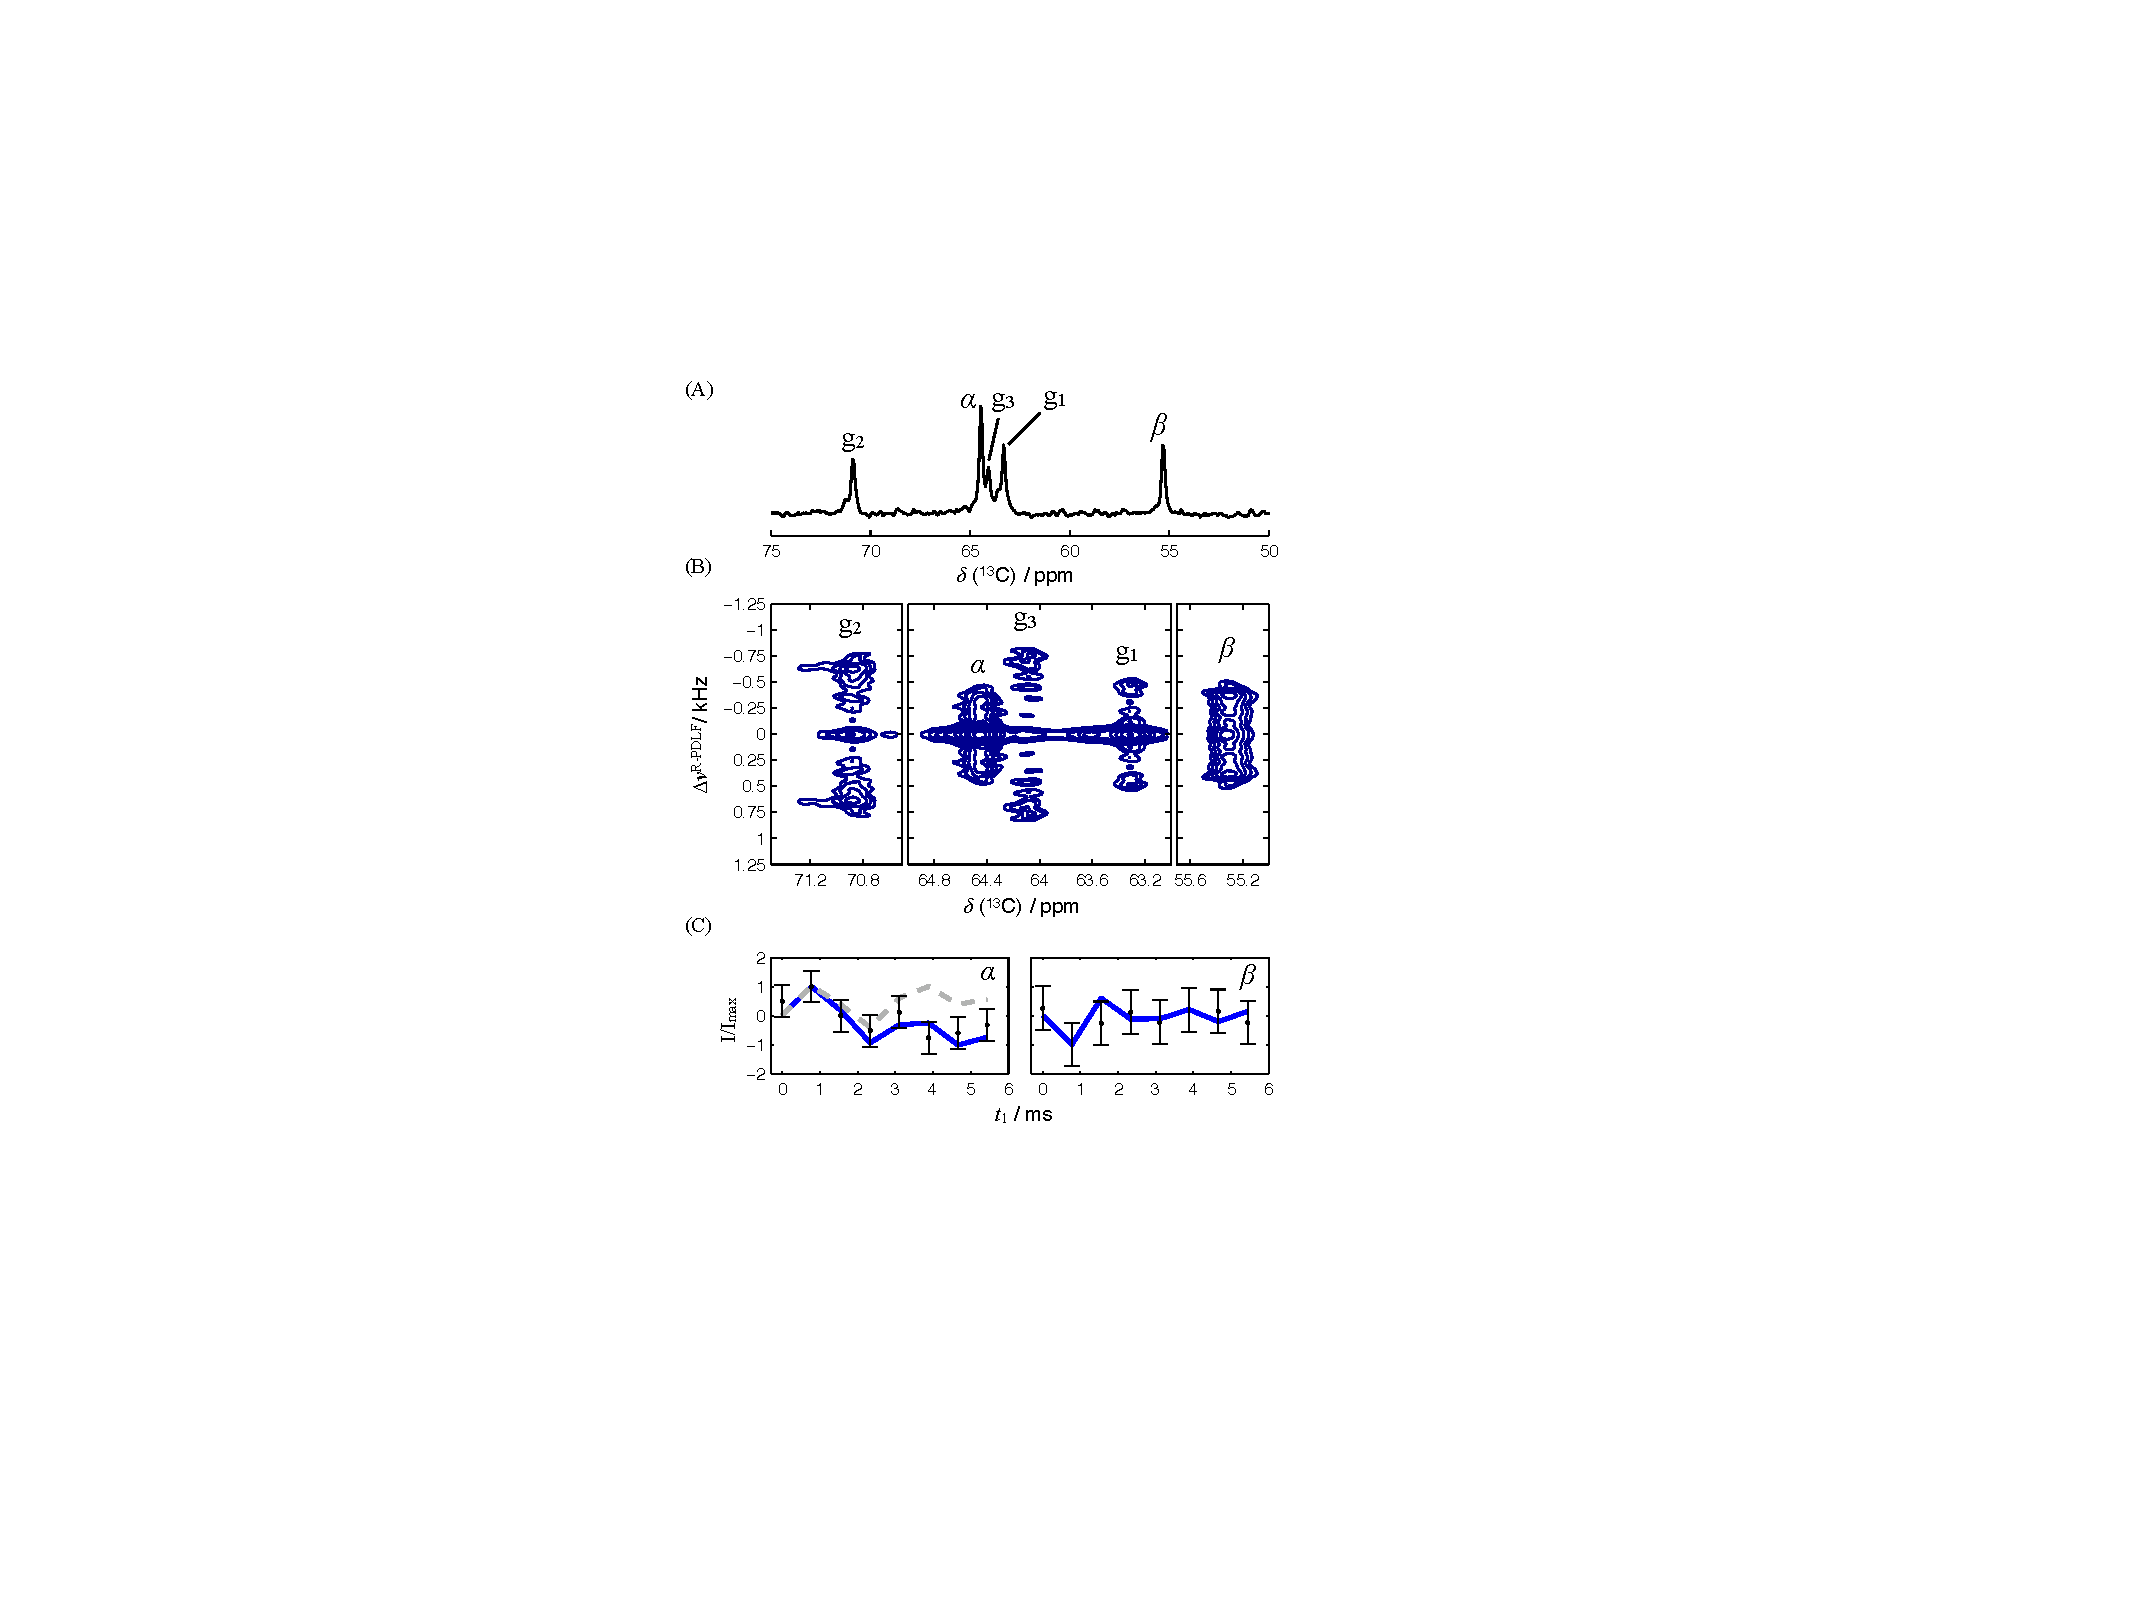
\includegraphics[width=8.5cm]{../Figs/fig1_POPS.pdf}
  \caption{\label{PShgSIGNSsimpson}
    The headgroup and glycerol backbone region of the (A) INEPT spectrum and
    (B) 2D R-PDLF spectra.
    (C) Experimental SDROSS data (points) and SIMPSON simulations (blue lines) with
    the order parameter values of -0.12 for the $\beta$-carbon, and 0.09 and -0.02
    for the $\alpha$-carbon slittings. The S-DROSS curve from SIMPSON simulation with positive value
    for the smaller $\alpha$-carbon order parameter (dashed grey).
  }
\end{figure}

The headgroup and glycerol backbone order parameters of 
POPS measured in this work are in good agreement with the previously reported
values from $^2$H NMR experiments of DOPS \cite{browning80} (Fig. \ref{HGorderParameters}).
When compared with the previously measured values for POPC \cite{ferreira13} (Fig. \ref{HGorderParameters}),
the $\beta$-carbon order parameter is significantly more negative and $\alpha$-carbon
experiences a significant forking in PS headgroup.
These features have been intepreted to arise from a rigid PS headgroup
conformation, stabilized by hydrogen bonds or electrostatic
interactions \cite{browning80,buldt81}, but detailed structrural interpretation is not
available. 
%The detailed structural differences between the headgroups is, however, not known.
\begin{figure}[]
  \centering
  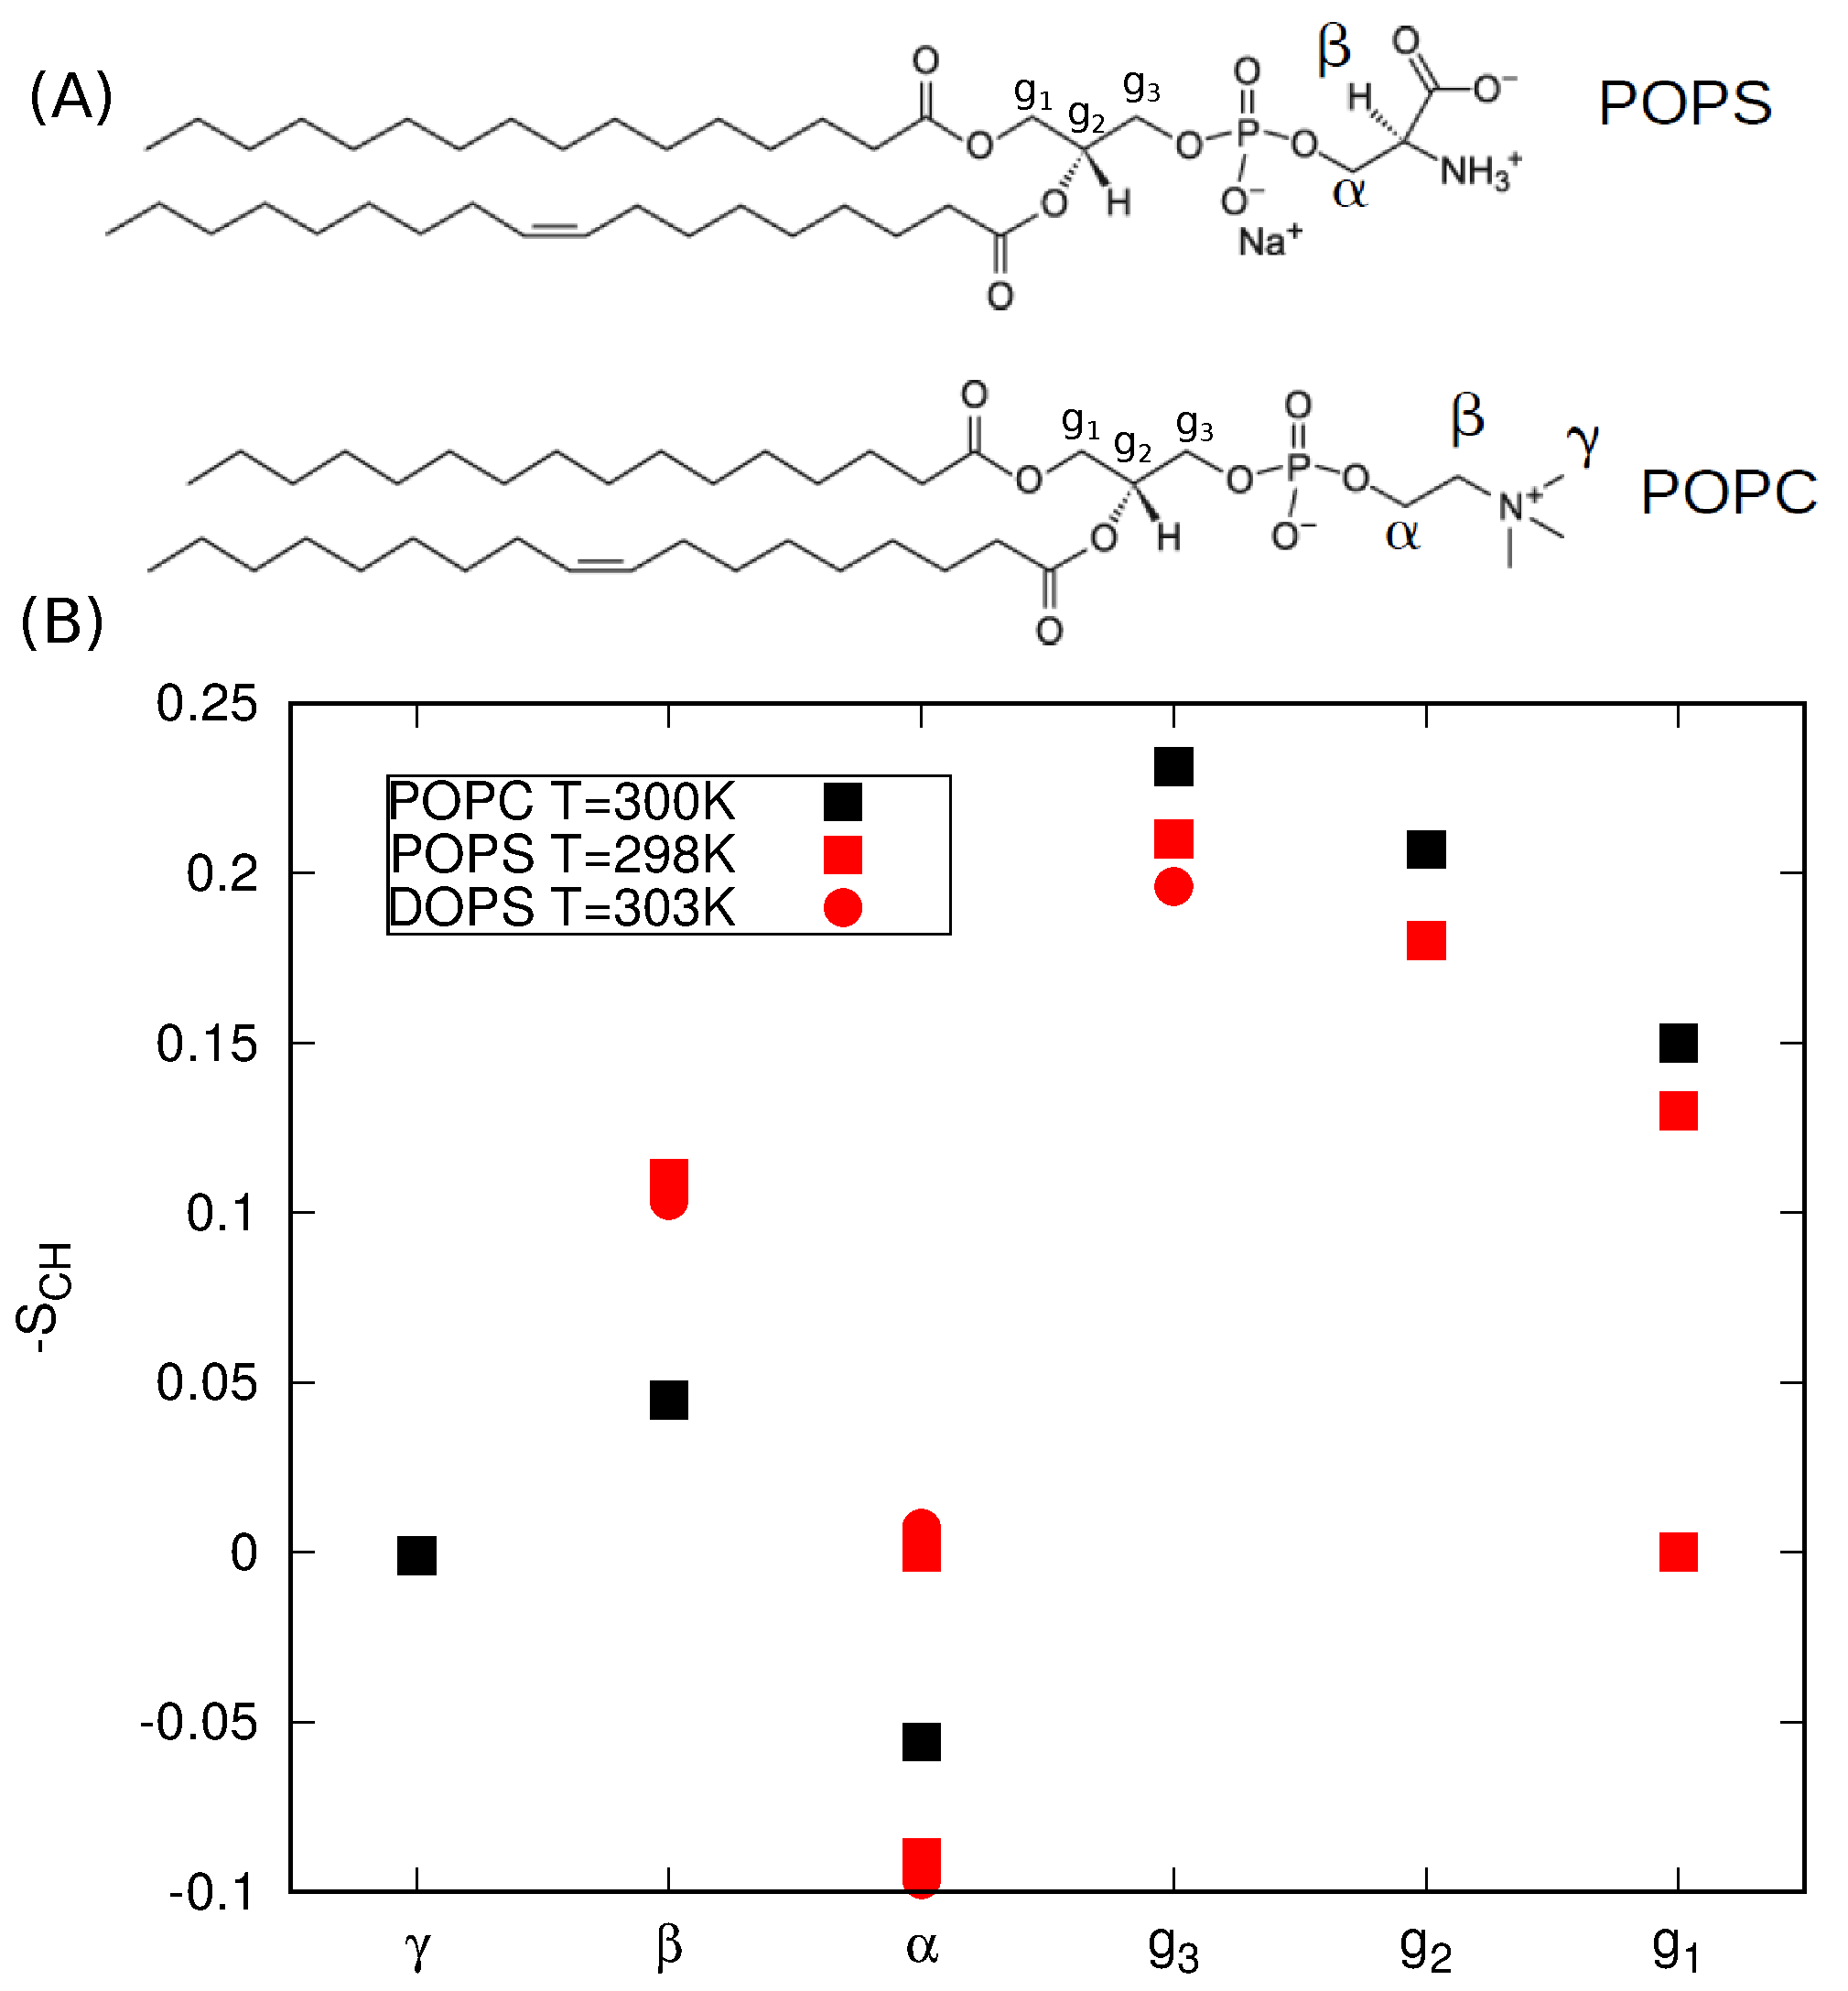
\includegraphics[width=9.0cm]{../Figs/PCPScomp.eps}
  \caption{\label{HGorderParameters}
    (A) Chemical structures and labels for the headgroup carbons.
    (B) Headgroup and glycerol backbone order parameters of POPS measured in this work compared
    with the values from DOPS ($^2$H NMR, 0.1M of NaCl) \cite{browning80} and 
    POPC  ($^{13}$C NMR) \cite{ferreira13} experiments. Signs of the PS order parameters
    are measured in this work. Signs of the PC order parameters are measured in Ref.~\cite{ferreira16}.
  }
\end{figure}


%\begin{figure}[]
%  \centering
%  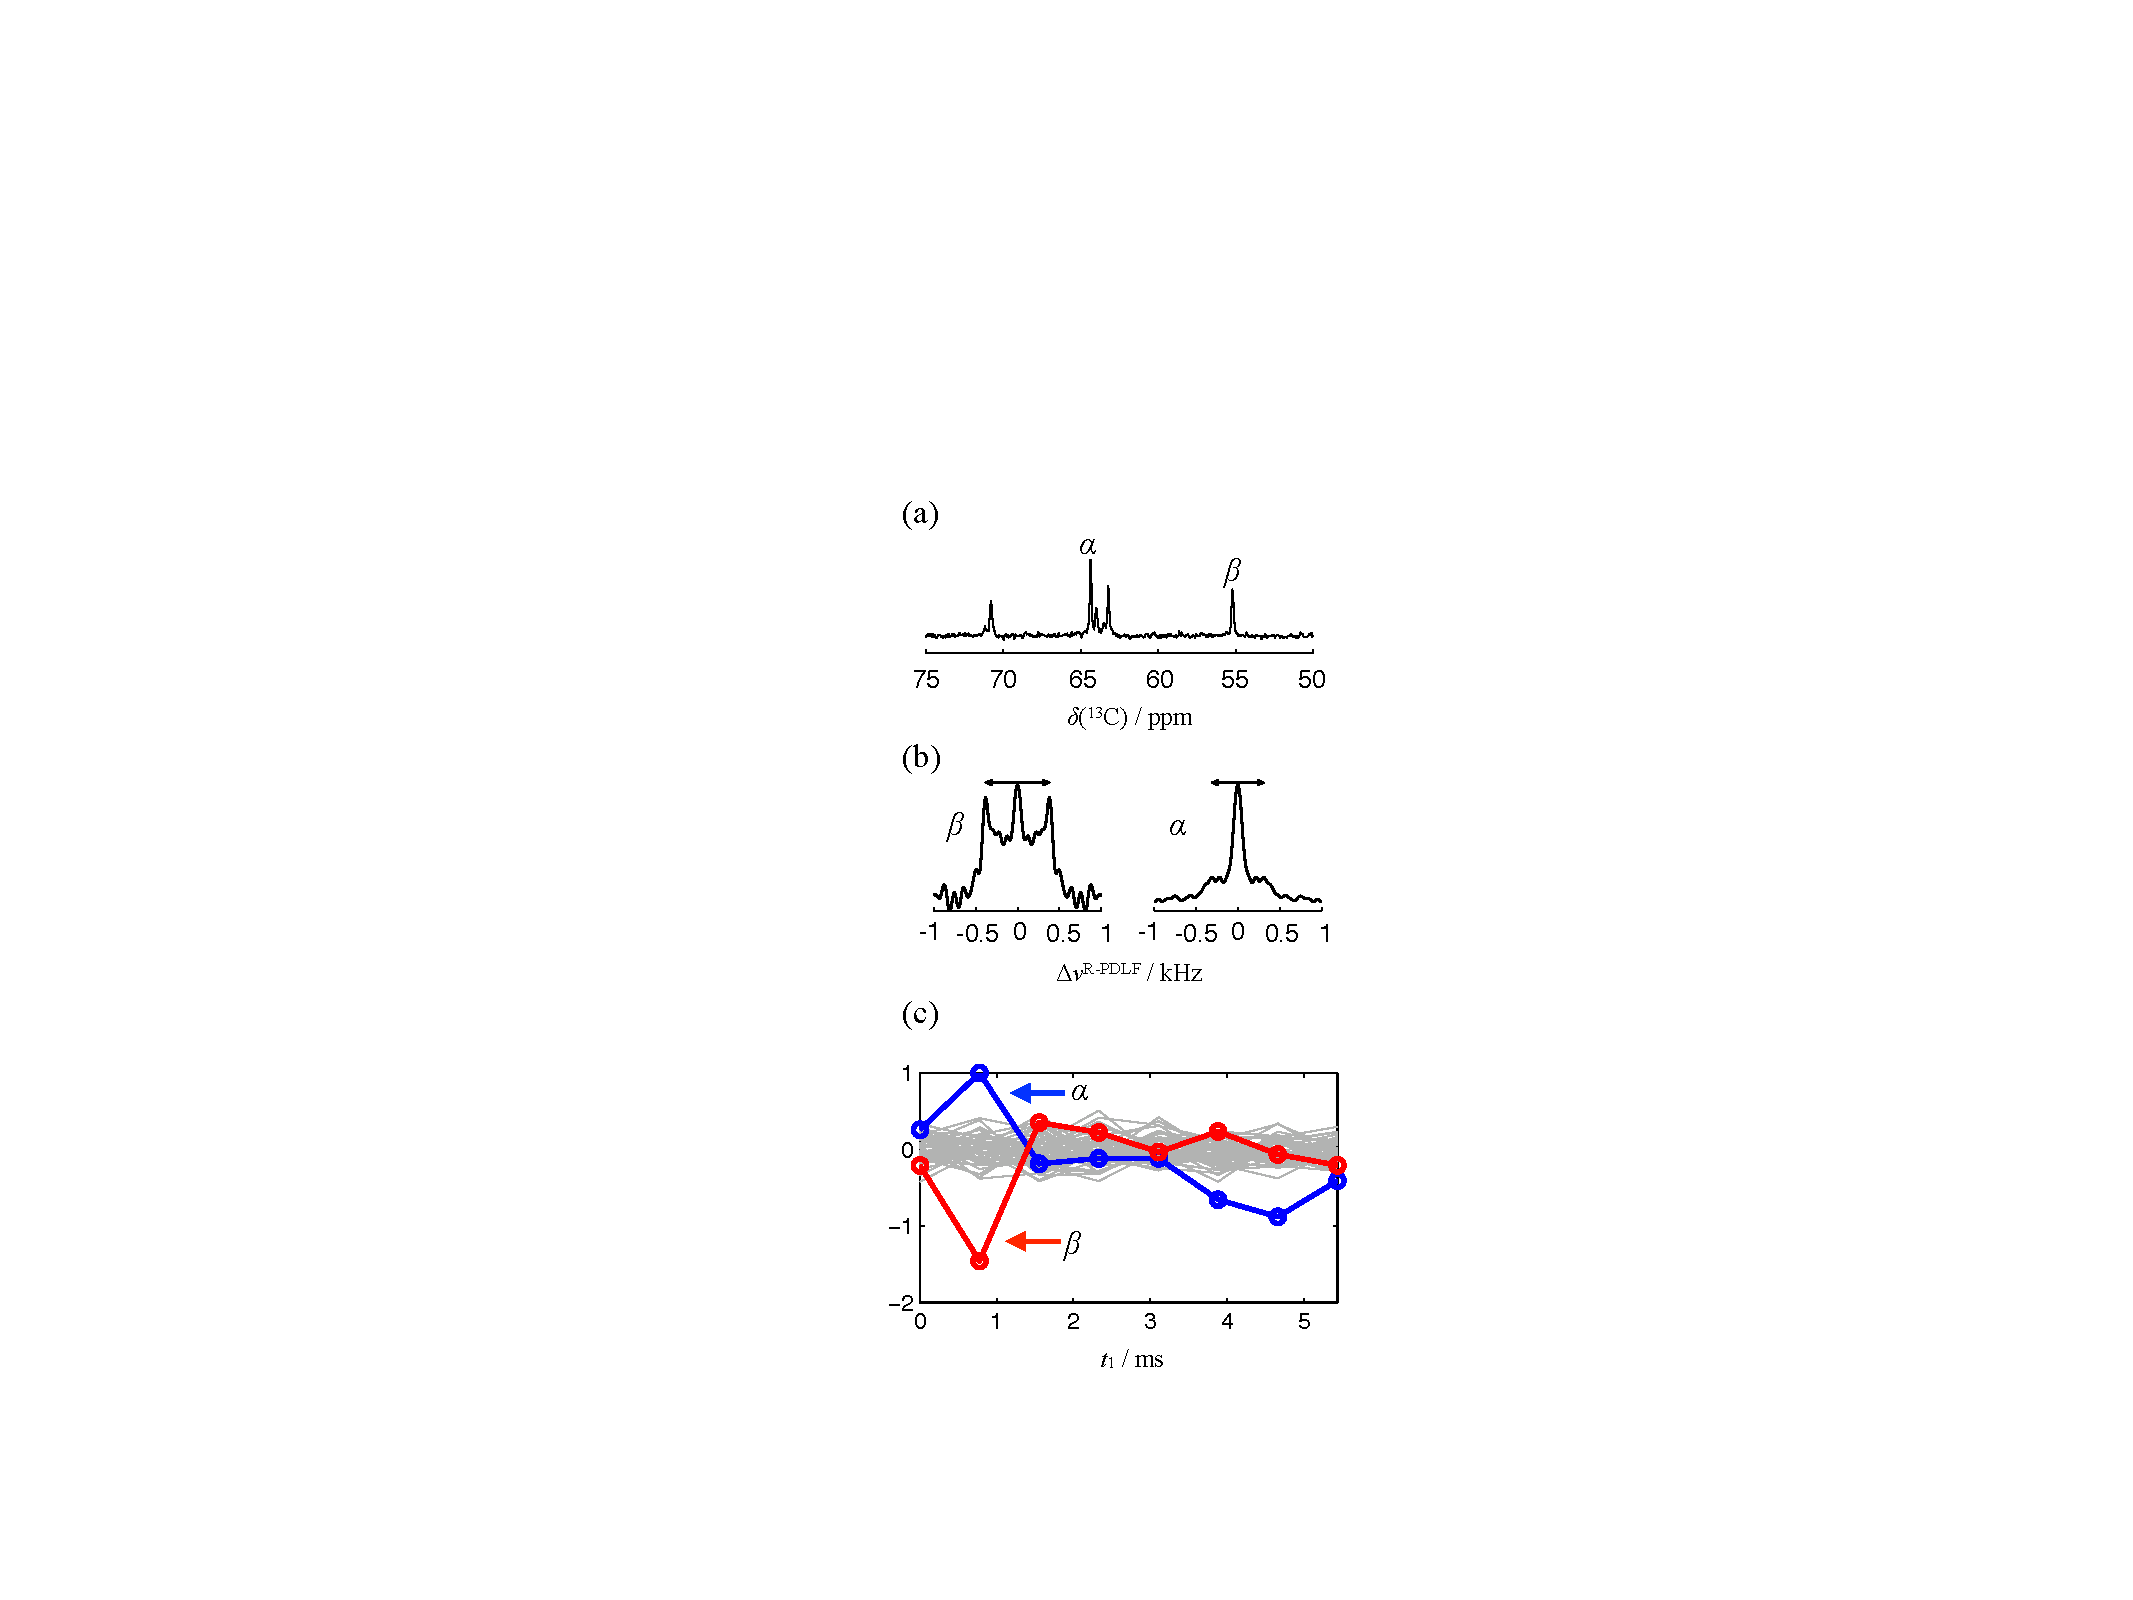
\includegraphics[width=9.0cm]{../Figs/PShgSIGNS.pdf}
%  \caption{\label{PShgSIGNS}
%    Experimental results for sign measurement for POPS sample
%  }
%\end{figure}


\subsection{Headgroup and glycerol backbone in simulations of PS lipid bilayers without additional ions}
\begin{figure}[]
  \centering
  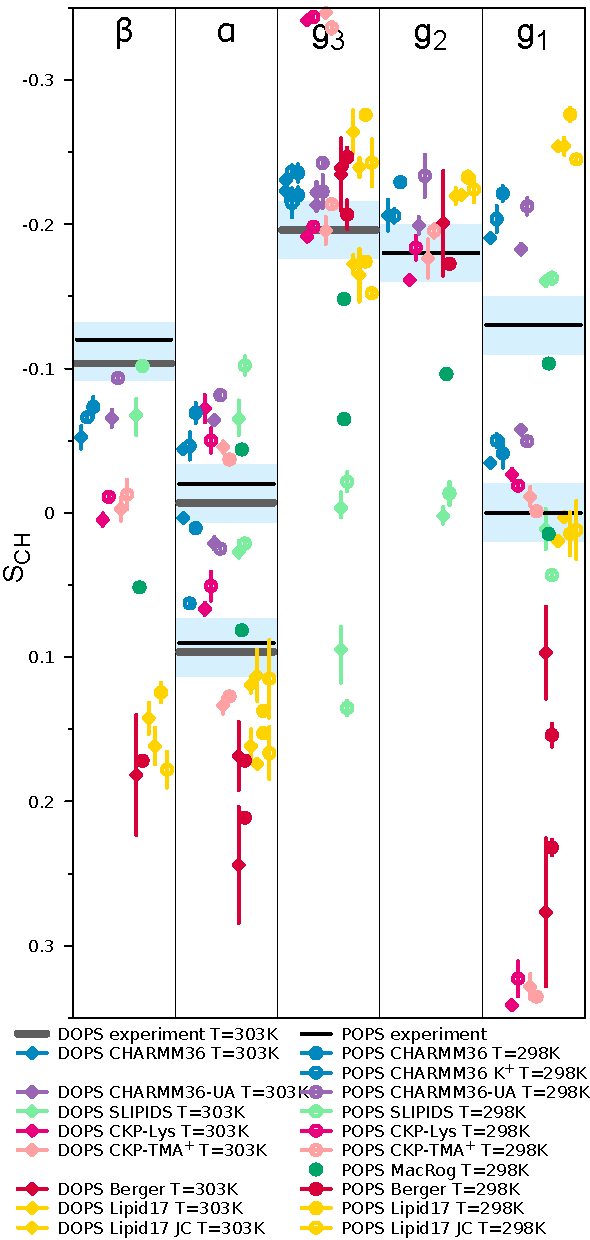
\includegraphics[width=9.0cm]{../Figs/HGorderparametersPS.pdf}
  \caption{\label{HGorderParametersPS}
    Order parameters for PS headgroup and glycerol
    backbone from simulations with different models and experiments without CaCl$_2$.
    All DOPS data at 303~K, POPS at 298~K.
    Experimental data from \cite{browning80} contain 0.1~M of NaCl.
    Signs are taken from experiments for POPS described in Supplementary Information.
    The vertical bars shown %for most computational values
    are not error bars, but demonstrate that %for these systems
    we had at least two data sets; the ends of the bars mark the extreme values from the sets, and the dot marks their measurement-time-weighted average.
  }
\end{figure}

\begin{figure}[]
  \centering
  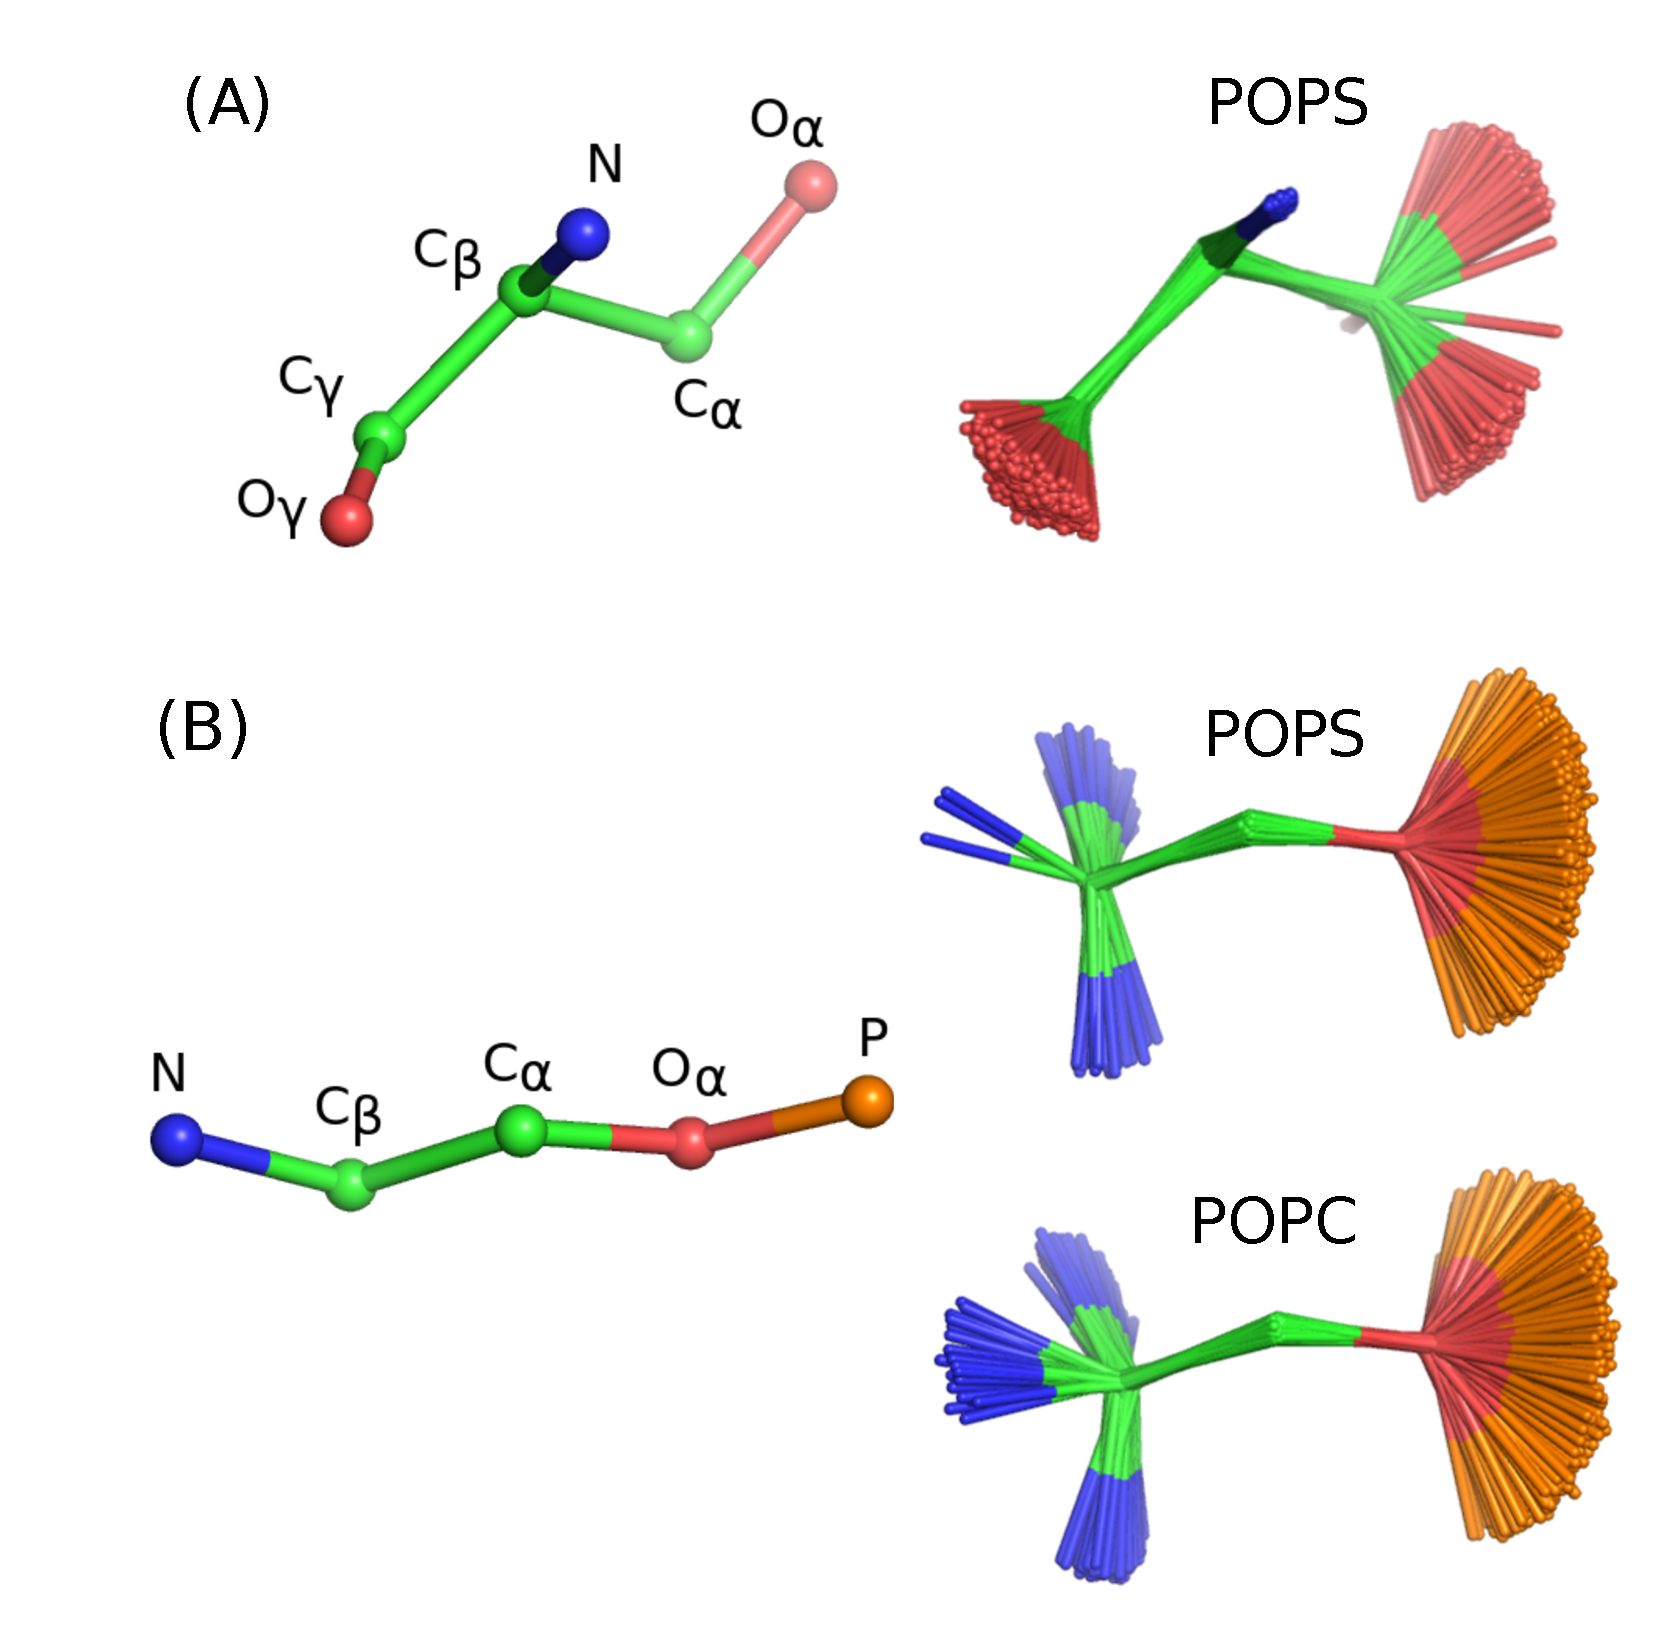
\includegraphics[width=9.0cm]{../Figs/structures.eps}
  \caption{\label{HGstructuresPSandPC}
    Overlayed snapshots from CHARMM36 simulations in best agreement with experiments
    to demonstrate the conformational fluctuations around
    a) C$_\alpha$-C$_\beta$-C$_\gamma$-O$_\gamma$ and  O$_\alpha$-C$_\alpha$-C$_\beta$-N
    of PS headgroup and b) N-C$_\beta$-C$_\alpha$-O$_\alpha$ and C$_\beta$-C$_\alpha$-O$_\alpha$-P
    dihedrals of PS and PC headgroups.
  }
  \todo{We need atom labeling for b). Similar to the one in a) would be good} \\
\end{figure}

\begin{figure}[]
  \centering
  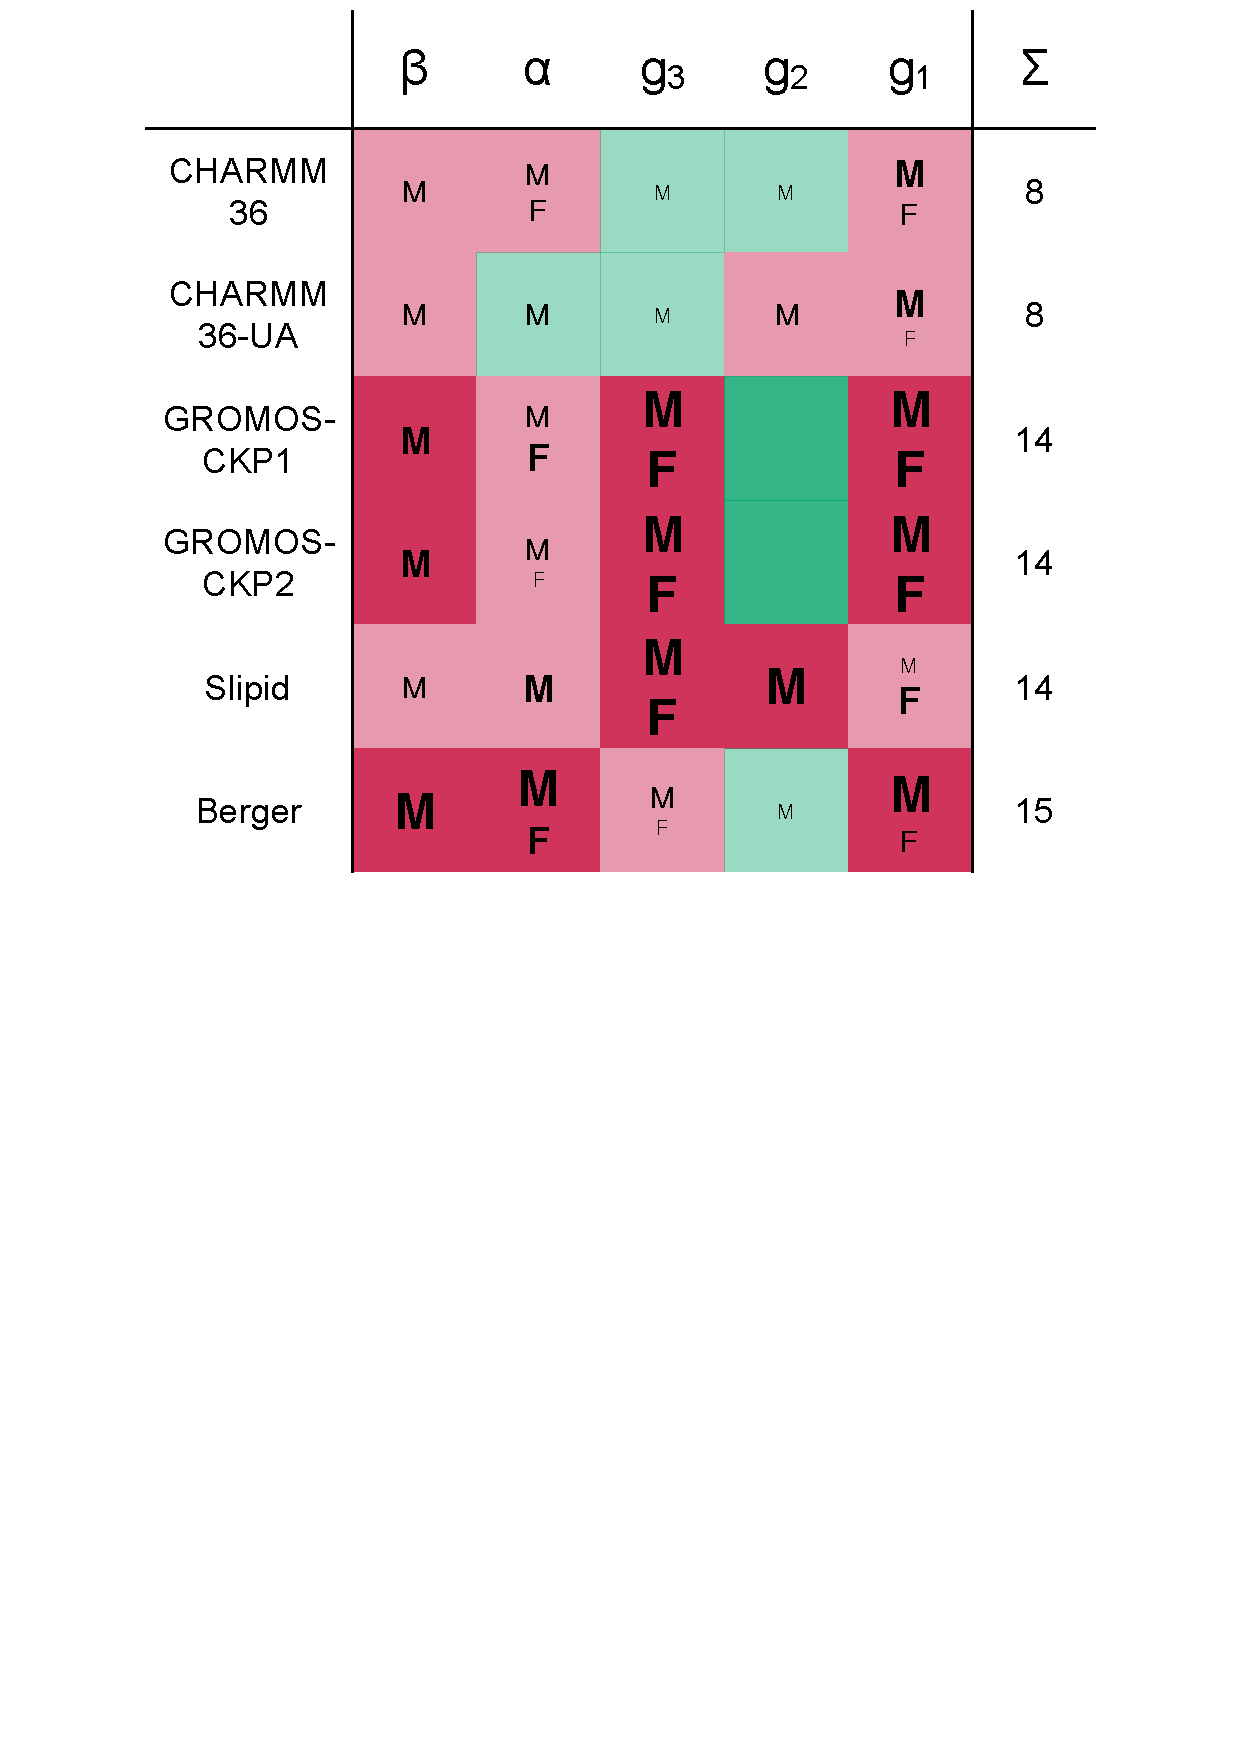
\includegraphics[width=9.0cm]{../Figs/comparisonTablePS.pdf}
  \caption{\label{comparisonTablePS}
    Rough subjective ranking of force fields based on Figure~\ref{HGorderParametersPS}.
    Here ÒMÓ indicates a magnitude problem, ÒFÓ a forking problem; letter size increases with problem severity. Color scheme: Òwithin experimental errorÓ (dark green), Òalmost within experimental errorÓ (light green), Òclear deviation from experimentsÓ (light red), and Òmajor deviation from experimentsÓ (dark red). The $\Sigma$-column shows the total deviation of the force field, when individual carbons are given weights of 0 (matches experiment), 1, 2, and 4 (major deviation). For full details of the assessment, see Supplementary Information.
  }
\end{figure}

The headgroup and glycerol backbone of PS lipids show wide variety between different simulation
models in the order parameters and structures (Figs. \ref{HGorderParametersPS} and \ref{HGandGLYstructuresPS}),
as previously observed also for PC lipids \cite{botan15}.
The models perform generally less well for PS lipids than for PC lipids in the previous study
(Figs.~\ref{HGorderParametersPS} and \ref{comparisonTablePS} vs. Figs. 2 and 4 in Ref.~\cite{botan15}).
Therefore, the interpretation of structural differences between PC and PS headgroups
from simulations is not straightforward.

The best performing models,
Slipids, CHARMM36 and CHARMM36ua, reproduce the larger forking of the $\alpha$-carbon 
and the Slipids model reproduces also the lower of the $\beta$-carbon order parameter
when comparing the PS results to PC (Fig. \ref{HGorderParametersPS} vs. Fig. 2 in Ref.~\citenum{botan15}).
Interestingly, the dihedral angle distributions of C$_\alpha$-C$_\beta$-C$_\gamma$-O$_\gamma$ show
a single narrow maximum close to 120$^{\circ}$ in the best three models, while other models give several maxima
in different locations (Fig. \ref{dihedralsHG}). The restricted motion is also
visible in the sampled conformations (Figs.~\ref{HGstructuresPSandPC} a) and \ref{HGandGLYstructuresPS})
suggesting that the rotation of carboxyl group is limited in the serine headgroup.
In addition, the CHARMM36 simulations, in best agreement with experiments for both lipids,
show more asymmetric and restricted N-C$_\beta$-C$_\alpha$-O$_\alpha$ dihedral distribution 
in PS headgroup than in PC (Figs.~\ref{HGstructuresPSandPC} b) and \ref{dihedralsHGpc}).
These results might manifest the increased rigidity anticipated in the early experimental studies \cite{browning80,buldt81}.
Also the dihedral distributions and sampled conformations of glycerol backbone region
significantly vary between different simulations models 
(Figs. \ref{dihedralsGLY}, \ref{HGandGLYstructuresPS}, \ref{dihedralsGLYpc} and \ref{HGandGLYstructuresPSPC}),
but further analysis is beyond the scope of this work which the PS headgroup.

The observed conformations of PS headgroup may be useful when interpreting experiments and
can guide the further force field development. However, more accurate simulations are
required to confirm the results because the simulated PS headgroup order parameters
are not within the experimental error bars in any of the tested models.


%
%The total deviation from the experiments ($\Sigma$ in Fig. \ref{comparisonTablePS})
%for the best performing CHARMM36 model is larger for PS lipids (8)
%than for PC (3) \cite{botan15}.



\subsection{Counterion binding and interactions between PC and PS headgroups}\label{ciBINDINGsection}
\begin{figure}[]
  \centering
  \includegraphics[width=9.0cm]{../Figs/NAdensPOPS.eps}
  \caption{\label{NAdensPOPS}
    Counterion densities of POPS lipid bilayer along the membrane normal from
    simulations with different force fields.
  }
\end{figure}

\begin{figure*}[ht]
  \centering
  \includegraphics[width=18cm]{../Figs/CHANGESwithCaClPS.eps}
  \caption{\label{changesWITHCaClPS}
    Changes of POPC (left) and POPS (right) headgroup order parameters from POPC:POPS (5:1) mixture
    as a function CaCl$_2$ concentration from experiments \citenum{roux90} and different simulations
    at 298K (except the data for Berger model is from simulation of POPC:POPS (4:1) mixture at 310K \cite{ollila07a,melcrova16}). 
    The order parameter values from systems without calcium are set as the zero point of y-axis,
    except for the $\alpha$-carbon order parameter of POPS (bottom, right) for which the both order parameters are shifted
    such that the lower order parameter is zero without additional ions to correctly illustrate
    the forking with different concentrations of calcium.
    Potassium counterions are used in MacRog simulations and sodium counterions in Lipid14/17 simulations.
    In CHARMM36 and Berger simulation with added calcium, the charge is neutralized with calcium and monovalent counterions are not present.
  }
  \todo{Upcoming simulations with original CHARMM36 have been mentioned in the blog:
  http://nmrlipids.blogspot.com/2017/12/nmrlipids-iv-current-status-and.html?showComment=1520090718976\#c5569269391707740056} \\
\end{figure*}

\begin{figure}[ht]
  \centering
  \includegraphics[width=9cm]{../Figs/CAdensPCPSmixture.eps}
  \caption{\label{CAdensPCPSmixture}
    Ca2+ density profiles from simulations.
  }
  \todo{The CHARMM results are mass densities, number densities should be used when the data by Jesper Madsen is available.} \\
  \todo{Should we include also counterions into the plot?} \\
  \todo{Figure needs general improvement.}
\end{figure}

Membranes containing PS lipids are always accomppanied with counterions which
modulate electrostatic interactions between lipids and other biomolecules. 
Counterions are also suggested to screen the repulsion between charged lipid headgroups 
in MD simulations and reduce the area per lipid of PS bilayers to be smaller than in PC
bilayers~\cite{pandit02,mukhopadhyay04,pedersen06}. 
The counterion density profiles along membrane normal 
show significant differences between simulation models in both binding affinity
and distribution of ions in the interface (Fig. \ref{NAdensPOPS}).
The experimental area per lipid (62.7 $\AA^2$) \cite{pan14} 
is reproduced only in Gromos-CKP simulations and in the MacRog simulation
with potassium counterions, while other models give significantly lower values (Fig. \ref{NAdensPOPS}).
The counterion binding and concomintant electrostatic screening of the headgroup
repulsion does not fully explain the low area per molecule values
because the MacRog simulation with strongest sodium binding
(the lowest concentrations in bulk water) gives the same area per molecule
as CHARMM36ua simulation with significantly weaker counterion binding
affinity.
%CHARMM36, CHARMM36ua and Slipid models give
%smaller area per lipid than Gromos-CKP models with similar counterion binding affinity.
On the other hand, changing counterions from sodium to potassium, having weaker binding
affinity, increases the area per molecule from 53 $\AA^2$ to 63 $\AA^2$ in MacRog simulations.
%with potassium counterions and weaker
%binding affinity give larger area per molecule 
%increasing counterion binding affinity reduces the area per molecule
%when comparing between sodium and potassium in 
%or between
%ff99 and jc ions in Lipid 17 simulations.
In conclusion, the results are in line with the previous study suggesting that the
low area per molecule in PS lipid bilayers originate from the combination
of both counterion binding and hydrogen bonding network between lipid
headgroups \cite{petrache04}.
%, Berger and Lipid17/JC simulations.
%Slipids, Berger, MacRog, and Lipid17 exhibit a clear single maxima in the
%counterion density, but slightly at different distances from the bilayer
%center. Other models exhibit more complicated distribution, often including
%two local maxima in the density profile.
%CHARMM36, CHARMM36ua and Gromos-CKP models exhibit two local maxima in counterion
%density, while a single maxima is observed in the other models. 



Binding of coions to zwitterionic PC lipid bilayers has been previously
evaluated against experiments using the changes of headgroup order parameters
as a function of ion concentration \cite{catte16}. This is less straighforward
for charged lipid bilayers because counterions are always present and the
ion free reference state does not exist.
In addition, the analysis is complicated by the artificial aggregation of counterions
in solution observed in some simulations (section \ref{mixtureTOadditionalCIs} in the supplementary information).
Here, we evaluate the amount of bound charge using the changes of
headgroup order parameters with increasing amount of negatively charged lipids in the bilayer.
According to the electrometer concept, the headgroup order parameters of POPC
increase when negativaly charged POPS lipids are incorporated in lipid bilayer
(section \ref{HGorderparametersPCvsPEPSPGchol})~\cite{seelig87,scherer87}.
This is reproduced in the MacRog simulations with potassium counterions having
the weakest binding affinity to POPS lipid bilayers (Fig.~\ref{NAdensPOPS}),
while other simulations predict no change or decrease in the order parameters
(Fig. \ref{HGorderparametersPCvsPS}).
%In experiments and MacRog simulations, the increasing amount of negative charge
%in the membrane tilts the PC headgroup more parallel to the membrane plane
%leading to the larger order parameters.
In Berger and CHARMM36 simulations, the stronger counterion binding cancel
the effect of negatively charged headgroups and the headgroup order parameters
do not increase with increasing amount of PS lipids.
%the order parameters decrease with the increasing amount of
%positive counterions of PS lipid.
%In CHARMM36 simulations, the counterion binding neutralizes the negative charge
%of lipids at the interface and 
Therefore, we suggest that the relatively weak binding of potassium
in the MacRog simulations (Fig. \ref{NAdensPOPS}) predicts the most
realistic surface charge density in membranes containing PS lipids,
while the other tested simulation models overestimate the counterion
binding affinity. The results are in line with the changes of headgroup order
parameters as a function of added counterions analyzed in section \ref{mixtureTOadditionalCIs}
in the supplementary information.
%reproduces the correct
%response of POPC headgroup to the increasing amount of negatively charged lipids,
%indicating that these simulations have 
\begin{figure*}[]
  \centering
  \includegraphics[width=16.0cm]{../Figs/HGorderparametersPCvsPS.eps}
  \caption{\label{HGorderparametersPCvsPS}
    Changes of PC (left panel) and PS (right panel) headgroup order parameters
    from POPC:POPS mixtures with increasing amount of POPS.
    Experimental results of POPC are taken from Ref. \citenum{scherer87}
    (signs are determined as discussed in \cite{botan15,ollila16}).
    Experimental values for POPS in pure bilayer and in mixture are  
    measured in this work and in Ref. \citenum{roux90} at 298K, respectively.
    Since the experimental data of POPS in pure and diluted mixture come from
    different experimental sets (13C NMR in this work and 2H NMR from Ref. \citenum{roux90}),
    the experimental change of the order parameter is less accurate than in typical measurements
    where same technique is used in all conditions, see discussion about qualitative and quantitative 
    accuracy in Ref. \citenum{ollila16}.
    For POPC (left panel) the zero point of y-axis is set to the value of pure bilayer.
    For $\beta$-carbon of POPS (right panel, top) the zero point of y-axis is
    set to the value from POPC:POPS (5:1) mixture.
    For $\alpha$-carbon of POPS (right panel, bottom) the y-axis is tranferred
    with the same value for both order parameters such that the lower order
    parameter value from POPC:POPS (5:1) mixture is at zero
    to correctly illustrate the significant forking.
  }
  \todo{Simulation of CHARMM36 at 298K should be maybe rerun with Gromacs 5.} \\
  \todo{The data from POPC used in Gromos-CKP by would be useful for this plot.}
\end{figure*}


The headgroup order parameteres of POPS shift closer to zero when bilayer
is diluted with POPC (Fig.~\ref{HGorderparametersPCvsPS}),
which is interpreted to indicate less rigid structure of PS headgroups in
the mixture~\cite{browning80,buldt81,roux90,roux91,scherer87}.
This shift is observed only in lipid14/17 simulations
%, the headgroup order parameters of POPS shift closer
%to zero when the bilayer is diluted with POPC,
but the numerical values of order parameters are too far from experiments, having also different signs,
for the proper interpretation of the experimental data.
In CHARM36 and Gromos-CKP simulations, the shift of headgroup order
parameters toward zero are not observed when bilayer
diluted with POPC (Fig. \ref{HGorderparametersPCvsPS}).
Therefore, we conclude that more accurate force fields are necessary
for MD simulation studies of PC-PS headgroup interactions.  
%The $\beta$-carbon order parameter
%increase with increasing amount of PS in CHARMM36 and MacRog simulations in contrast
%to the experimental data.
%The smaller $\alpha$-carbon order parameter increase in both
%simulation models with increasing amount of PS, while it is almost unchanged in experiments.
%The larger $\alpha$-carbon order parameter increase in MacRog and decrease in CHARMM36
%with increasing amount of PS, both model exhibiting a poor agreement with experiments. 

%Therefore, the intermolecular interactions at the headgroup region seems
%to be important for the physical properties of mixed lipid bilayers.
%These interactions can be indirectly monitored by measuring the
%headgroup order parameters from PS:PC mixtures with different molar
%ratios.



\subsection{Ca$^{2+}$ binding affinity to bilayers with negatively charged PS lipids}


Ion binding affinity to membranes containing negative charged PS lipids can be
measured by detecteding the PC lipid headgroup order parameters
from POPC:POPS (5:1) mixtures (section~\ref{electrometerFORmixtures}),
where the dehydrated lipid-ion complexes and phase separation are 
not observed~\cite{feigenson86,mattai89,roux90,roux91}.
As expected from the previous study of pure PC lipid
bilayers \cite{catte16}, almost all the tested simulation models overestimate the decrease of
POPC headgroup order parameters as a function of Ca$^{2+}$ concentration in POPC:POPS (5:1) mixtures 
with respect to the experiments \cite{roux90} (Fig. \ref{changesWITHCaClPS}), indicating overestimated
calcium binding binding affinity. Only exception is the CHARMM36 model with the NBfix
interaction employed for calcium~\cite{kim16}, which underestimates the order parameter changes
indicating weaker binding affinity than experiments.
%incorporated in the parameters give by the CHARMM-GUI at the time of running the simulations (January 2018),
Notably, CHARMM36 simulations with NBfix corrections \cite{venable13,kim16} give similar binding affinities of
calcium and sodium to POPC bilayer (see section \ref{CHARMMcalciumNBfix}), in contrast to the experimental 
data~\cite{cevc90,akutsu81,altenbach84}. Therefore, we conclude that the calcium binding affinity,
manifested by the peaks in the density distributions along membrane normal (Fig. \ref{CAdensPCPSmixture}),
is underestimated in CHARMM36 simulations with the NBfix for calcium \cite{kim16} but overestimated 
in all the other tested models.

%It should be noted, however, that the lowest concentration (100mM) gives
%a good agreemet with experiments
%\todo{Should be analyze/discuss this further?
%  Binding with $\sim$100 mM is saturated in both Berger and MacRog simulations. Maybe this is realistic?
%It should be noted that Berger simulation do not have counterions.}.


The headgroup order parameters of POPS measured from POPC:POPS (5:1) mixture
exhibit a strong dependence of CaCl$_2$ with small concentrations and rapid saturation
below 100 mM (Fig. \ref{changesWITHCaClPS}).
The order parameter of POPS $\beta$-carbon increase and the larger $\alpha$-carbon 
decrease with the added CaCl$_2$ in experiments. Slight increase is observed in
the smaller $\alpha$-carbon. All the changes are significantly overestimated in the
tested simulation models, including the CHARMM36 with the NBfix for calcium \cite{kim16},
where the binding affinity was underestimated. 
In addition, different simulation models predict qualitatively different behaviour
for the POPS $\alpha$-carbon order parameters with the added calcium.
For example, both order parameters decrease in Berger simulations but increase
in MacRog simulations, while behaviour in Lipid14/17 and CHARMM36 simulations is
more complicated. This is in contrast to the PC headgroup, where
qualitatively correct reponse to the bound ions is observed
in all simulation models despite of the significant discrepancies in the headgroup
structure without additional ions~\cite{catte16}. Therefore, we conclude that
the improvement of force fields is necessary to correctly describe interactions between
PS headgroup and calcium ions using MD simulations.
%The response of POPS headgroup order parameters to the bound charge is systematic but
%less well understood than the responce of PC headgroups used in the electrometer
%concept \cite{seelig87,roux90}.



\section{Conclusions}
We have collected a set of experimental NMR order parameter data,
which could be combined with MD simulations to interpret the
headgroup structure and cation binding details to negatively charged
membranes containing PS lipids. Using open collaboration method, we
tried to find a MD simulation model which would be sufficiently accurate
to interpret the experimental data. However, none of the tested models
was accurate enough. In line with the previous study for PC lipids \cite{catte16},
MD simulation models seems to generally overestimate cation binding also
to negatively charged bilayers containing PS lipids, with some exceptions.
The response of PS lipid headgroup order parameters to the bound cations
does not agree with experiments, even in the cases where binding affinity is
not overestimated. This is in contrast to the previous results with PC lipids,
where the qualitative response of the headgroup order parameters was in agreement
with experiments even in the cases where the headgroup structure without ions was not
correct and the cation binding affinity was overestimated. In addition, the inaccurate
responses of PS headgroup order parameters to the dilution with PC lipids suggests
that the PC-PS interactions are not accurately described by the tested models.

Our results pave the way for improving the PS lipid parameters for MD simulations
by offering the set of experimental data for the quality measurement, by
pinpointing problems areas in the models and suggesting directions for the corrections.
Improvements using the electronic continuum correction is already in progress \url{https://github.com/jmelcr/ecc_lipids},
following the recent work for PC lipids \cite{melcr18}.

% Tables may be be put in the text as floats.
% Here is an example of the general form of a table:
% Fill in the caption in the braces of the \caption{} command. Put the label
% that you will use with \ref{} command in the braces of the \label{} command.
% Insert the column specifiers (l, r, c, d, etc.) in the empty braces of the
% \begin{tabular}{} command.
%
% \begin{table}
% \caption{\label{} }
% \begin{tabular}{}
% \end{tabular}
% \end{table}

% If you have acknowledgments, this puts in the proper section head.
\begin{acknowledgments}
% Put your acknowledgments here.
\end{acknowledgments}

\newpage


% Create the reference section using BibTe
\bibliography{refs.bib}

%\newpage
%\section{APPENDIX: The NMR results reported by Tiago Ferreira}

\listoftodos

\end{document}
%
% ****** End of file aiptemplate.tex ******
